\documentclass[a4paper, 12pt]{article}

\usepackage{fontspec}   %加這個就可以設定字體
\usepackage{xeCJK}      %讓中英文字體分開設置
\usepackage{zhnumber}
\usepackage{indentfirst}
\usepackage{listings}
\usepackage{float}
\usepackage{graphicx}
\usepackage{caption}
\usepackage{fancyhdr}
\usepackage{hyperref}
\usepackage{amsmath}
\usepackage{multirow}
\usepackage[dvipsnames]{xcolor}
\usepackage{graphicx}
\usepackage{subcaption}
\usepackage{etoolbox}
\usepackage{tcolorbox}
\usepackage{multicol}
\usepackage{tabularx}
\usepackage[toc]{appendix}
\usepackage{titlesec}
\usepackage{titling}
\usepackage{newunicodechar}
\usepackage{hhline}
\usepackage{tocloft} % adding the tocloft package for toc customization

\usepackage[english]{babel}
\usepackage[autostyle]{csquotes}

\usepackage[sorting=nty]{biblatex}


\renewcommand\appendixtocname{附錄}


\addbibresource{ref.bib}

\setcounter{tocdepth}{5}
\setcounter{secnumdepth}{5}

\renewcommand\tabularxcolumn[1]{m{#1}}% for vertical centering text in X column
\newcolumntype{Y}{>{\centering\arraybackslash}X}


\usepackage[
  top=2cm,
  bottom=2cm,
  left=2cm,
  right=2cm,
%  headheight=17pt, % as per the warning by fancyhdr
%  includehead,
  includefoot,
  heightrounded, % to avoid spurious underfull messages
]{geometry} 

\newcounter{mysec}[section]
\renewcommand\thesection{%
    \addtocounter{mysec}{1}%
    \zhnum[style={Traditional,Financial}]{mysec}、}
\renewcommand\thesubsection{\zhnum{subsection}、} % added a 、
\renewcommand\thesubsubsection{(\zhnum{subsubsection})} % added parentheses
% (full-width, don't know if that's what you want)
\renewcommand\theparagraph{} % you don't want paragraph numbers
\renewcommand\thesubparagraph{} % nor subparagraph numbers

% we have to adjust the spacing in the toc because the section label is longer than usual
\addtolength\cftsecnumwidth{1em}
\addtolength\cftsubsecindent{1em}
\addtolength\cftsubsubsecindent{1em}

% here we need to make sure the normal section counter is accessed
\titleformat{\section}{\Large\bfseries\filcenter}
    {\zhnum[style={Traditional,Financial}]{section}、}{.5em}{}
% not really sure what you intend to achieve with \fontsize but I'll leave it here
\titleformat*{\subsection}{\fontsize{12}{12}\bfseries} 
\titleformat*{\subsubsection}{\fontsize{12}{12}\bfseries}

% no extra version for numberless is necessary since no numbers are used anyways
% also you get newlines from omitting the [display] in \titleformat already
\titleformat{\paragraph}
    {\fontsize{14}{14}\bfseries}{}{0em}{} 
\titleformat{\subparagraph}
    {\fontsize{12}{12}\bfseries}{}{0em}{}
% we need the following so that they don't indent (second argument, 0em);
% you'll have to adjust the spacing though since this is not display style anymore:
\titlespacing*{\paragraph}{0em}{3.25ex plus 1ex minus .2ex}{.75ex plus .1ex} 
\titlespacing*{\subparagraph}{0em}{3.25ex plus 1ex minus .2ex}{.75ex plus .1ex}

\renewcommand{\maketitlehooka}{\sffamily}

\renewcommand{\baselinestretch}{1.5}

\pagestyle{fancy}
\renewcommand{\headrulewidth}{0pt}
\fancyfoot{}
\fancyhead{}
\cfoot{\footnotesize \thepage}


\addto\captionsenglish{%
  \renewcommand\appendixname{附錄}
  \renewcommand\appendixpagename{附錄}
  \renewcommand{\contentsname}{目錄}
  \renewcommand{\figurename}{圖}
}

\captionsetup[table]{name=表}
%\lhead{利用VAE-pix2pix生成擬真的山脈模型}
%\rhead{2021臺灣國際科學展覽會研究報告}

%\rfoot{李杰穎}

\lstset{basicstyle=\ttfamily, keywordstyle=\bfseries}

\setCJKmainfont{Noto Serif CJK TC}
\setmainfont{Times New Roman}
% \setmonofont[Color={0019D4}]{Consolas}
\setmonofont{Cascadia Code}
\XeTeXlinebreaklocale "zh"             %這兩行一定要加,中文才能自動換行
\XeTeXlinebreakskip = 0pt plus 1pt     %這兩行一定要加,中文才能自動換行
\title{利用VAE-pix2pix生成擬真的山脈模型}
\author{程品奕、李杰穎}
% \date{中華民國} %不要日期

\setlength{\parindent}{2em}
\setlength{\parskip}{0.5em}


\renewcommand{\thefootnote}{\roman{footnote}}

\begin{document}

\pagenumbering{roman}

\tableofcontents
\newpage

\begin{abstract}
    In this study, we use NASA's SRTM 1 Arc-second dataset to collect altitude maps from around the world, and we also use MapTiler API to collect corresponding satellite images. We use these collected images to train our VAE-pix2pix model, which is a Variational Autoencoder (VAE) combined with pix2pix (a Conditional Generative Adversarial Network). VAE-pix2pix can add details of the veritable mountain should have (including sharp ridges, mountain wall textures, continuous river networks, etc.) To the height map, which is drawn by users. Our model can generate the corresponding satellite images as well. Compared with the original pix2pix model, our model can generate heightmap and satellite images that are more realistic. Our model can also generate different styles of heightmap and satellite images by changing the value of the latent code, such as the color of the landform or the height of the snow line, which increases the diversity of the images generated by the model. To make our model can be better used, we have developed a client on Unity, which can generate a mesh that allows users it when developing the game in Unity. In conclusion, our work has simplified generating a realistic mountain model in-game or other fields as well.
\end{abstract}

\renewcommand{\abstractname}{摘要}
\begin{abstract}
    本研究利用NASA的SRTM 1 Arc-Second資料集\cite{srtm1arc}來收集全球各地的地形高度圖(heightmap),我們也利用了MapTiler網站收集了相對應的衛星空照圖。利用這些收集的圖像,訓練我們自行研究的VAE-pix2pix模型。VAE-pix2pix為Variational Autoencoder (VAE)及pix2pix (為一個Conditional Generative Adversarial Network)結合的模型,能將人工繪製的高度圖加上真實山脈應有的細節(包含尖銳的山脊、山壁上的紋路、連續的河流網路等……),也能生成出相對應的擬真衛星空照圖。相較於原pix2pix模型,VAE-pix2pix所生成的高度圖及空照圖會更接近於真實世界的山脈高度圖及空照圖,同時VAE-pix2pix模型也可以透過改變latent code的數值來生成出不同風格的高度圖及空照圖,如地貌的顏色或雪線的高度等,這些都增加模型生成圖像的多樣性。為了使我們建構的模型能廣泛的被應用,我們在Unity上開發了Unity客戶端,其生成的mesh可以讓使用者直接應用於遊戲的場景,簡化了生成擬真山脈模型的任務。
\end{abstract}

\newpage
\pagenumbering{arabic}

\section{前言}
\subsection{研究動機}
隨著3C的普及,遊戲已經成為現代人打發時間、舒壓及社交的必需品;隨著科技技術的進步,對於遊戲畫質的要求也越高,而在製作各種遊戲時,常常會需要生成擬真的地形作為場景。

傳統上,遊戲的擬真的山脈地形是透過人工繪製。在將大致的架構畫出來後,還需花費不少時間捏出山脊和挖出河流等細節部分。而近年來,人工智慧的演算法在圖像的生成上面有重大的突破,不論是憑空產生圖片或是將影像的風格提取出來,並轉換到另一張影像,都已經是可行的方法,因此本研究希望簡化人工繪製的過程,透過訓練生成對抗網路來達到生成擬真山脈地形的成果。

\subsection{研究目的}
本研究期望能簡化遊戲製作者在生成擬真的山脈地形的流程,同時確保生成擬真山脈的效果。研究參考遊戲地圖製作流程,是先產生高度圖(山脈、河流等地形特徵)再把衛星空照圖(植被、河流等地貌景觀)作為貼圖紋理貼到高度圖模型上。本研究使用兩個模型產生完整的擬真的山脈地形:

\begin{itemize}
    \item 地形擬真模型能有效地將人工設計的山脈架構高度圖自動轉換成擬真山脈地形高度圖。
    \item 貼圖模型則依地形擬真模型生成出的擬真高度圖,生成相對應的空照圖,作為擬真高度圖3D渲染時的貼圖紋理。
\end{itemize}

\section{研究過程與方法}
\subsection{文獻探討}
\subsubsection{物理侵蝕模型}
一般來說,若要提升遊戲中山脈地形的真實度,其中一種方法為使用侵蝕的物理模型,如論文\cite{jako2011fast},建構一個物理模型,模擬水流在地形上侵蝕與堆積,論文作者藉由此模型結合GPU,實現改變地形樣貌的效果。

根據論文\cite{jako2011fast}的內所敘述的物理模型,本研究利用PyTorch實現論文\cite{jako2011fast}所述之物理侵蝕模型,之後會將其與經訓練的VAE-pix2pix模型進行真實度及實用性的比較。

此物理侵蝕模型將地表分成正方形的網格,使用歐拉法求地表上每格的水深、含沙量和網格間的水流速,並根據水量和流速進行侵蝕和堆積,疊代多次後可得出侵蝕一段時間後的地面和水面高度圖。一次疊代的步驟如下:

\begin{enumerate}
    \item 在每個網格加上等量的水,模擬均勻的降雨
    \item 更新流速(加速度受坡度和阻力影響)
    \item 根據流速讓水流到鄰近的格子,同時搬運等比例的砂土
    \item 根據水量和流速進行侵蝕,增加水中含沙量,降低地面高度
    \item 將水中一定比例的沙土堆積到地面
    \item 移除每格一定比例的水,模擬蒸發
\end{enumerate}

\begin{table}[htbp]
    \centering
    \caption{\label{tab:para.}侵蝕模型的參數}
    \begin{tabularx}{\linewidth}{|Y|Y|Y|}
        \hline
        \textbf{參數}   & \textbf{說明}                & \textbf{數值} \\ \hhline{|=|=|=|}
        \texttt{KRain}  & 單位時間、面積的雨量         & $0.05$        \\ \hline
        \texttt{A}      & 水流速的乘數                 & $1$           \\ \hline
        \texttt{KS}     & 侵蝕速率                     & $30$          \\ \hline
        \texttt{drag}   & 水受到的阻力                 & $0.01$        \\ \hline
        \texttt{deltaT} & 一次疊代的時間步長           & $0.01$        \\ \hline
        \texttt{KD}     & 水中每單位時間沉澱的沙土比例 & $0.002$       \\ \hline
        \texttt{KE}     & 蒸發速率                     & $0.0002$      \\ \hline
    \end{tabularx}
\end{table}


調整表~\ref{tab:para.}~的變數能改變侵蝕後地形的風格。
為了使用戶可以調整河流的連續性,本研究在論文\cite{jako2011fast}的基礎上加入drag參數。而當drag越高時,河流越不連續,執行結果圖~\ref{fig:1}~與圖~\ref{fig:2}~。

\begin{figure}[htbp]
    \begin{subfigure}{0.45\textwidth}
        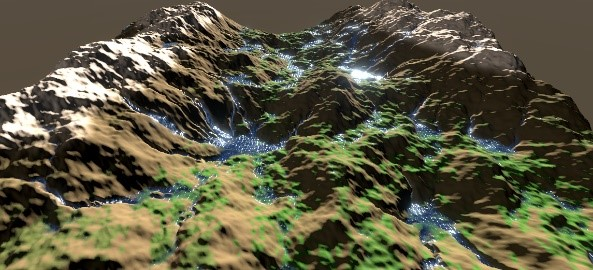
\includegraphics[width=\linewidth]{fig/1a.jpg}
        \caption{} \label{fig:1a}
    \end{subfigure}%
    \hspace*{\fill}   % maximize separation between the subfigures
    \begin{subfigure}{0.45\textwidth}
        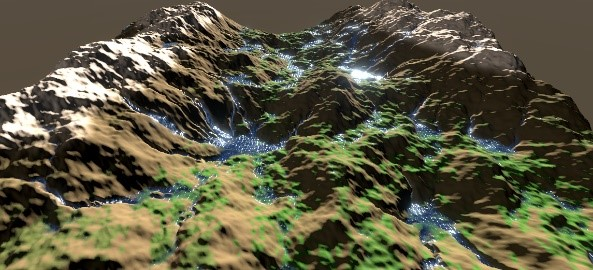
\includegraphics[width=\linewidth]{fig/1a.jpg}
        \caption{} \label{fig:1b}
    \end{subfigure}%
    \caption{drag的值對河流連續性的影響。(a) drag = 0、(b) drag = 0.2} \label{fig:1}
\end{figure}

\begin{figure}[htbp]
    \begin{subfigure}{0.45\textwidth}
        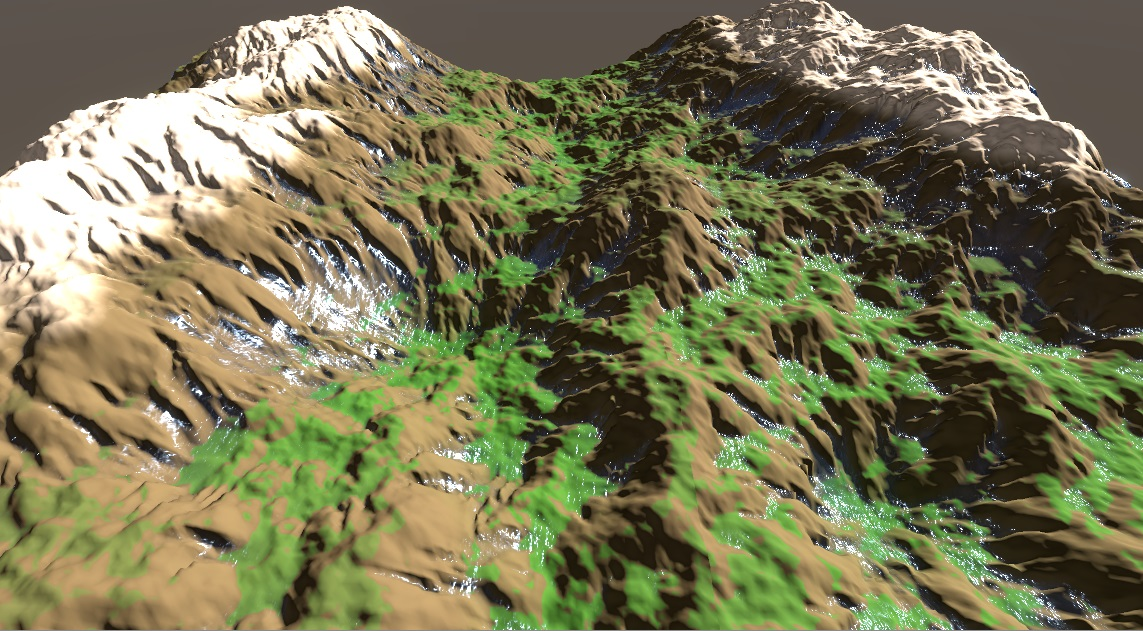
\includegraphics[width=\linewidth]{fig/2a.jpg}
        \caption{} \label{fig:2a}
    \end{subfigure}%
    \hspace*{\fill}   % maximize separation between the subfigures
    \begin{subfigure}{0.45\textwidth}
        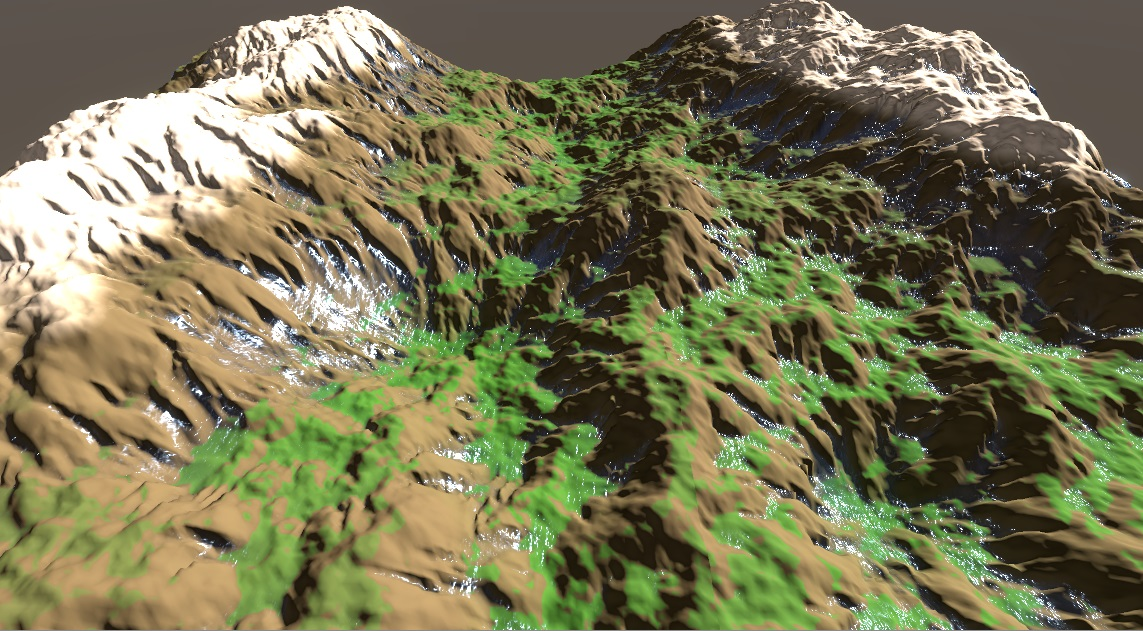
\includegraphics[width=\linewidth]{fig/2a.jpg}
        \caption{} \label{fig:2b}
    \end{subfigure}%
    \caption{參數A的不同會影響所產生的地形風格。(a) A = 0.1、(b) A = 1} \label{fig:2}
\end{figure}

\subsubsection{pix2pix模型}
論文\cite{isola2017image}則為pix2pix,是一個Conditional adversarial networks(又稱 Conditional GAN),其訓練時將一對影像當作輸入,而模型的目標則是將第一張圖片轉換為第二張圖片。例如圖~\ref{fig:3}~,模型的目標是將左圖做為輸入,輸出右邊的圖像。

\begin{figure}[htbp]
    \centering
    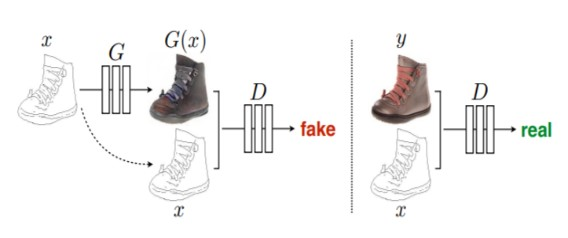
\includegraphics[width=\linewidth]{fig/3.jpg}
    \caption{pix2pix可做到的圖像風格轉換(取自\cite{isola2017image})}
    \label{fig:3}
\end{figure}

pix2pix由generator和discriminator兩個部分組成。generator的結構為U-Net,訓練時會嘗試把輸入圖像轉換為目標圖像。discriminator則是一個分類器,訓練時會嘗試分辨哪些圖是generator生成的圖,哪些是真的目標圖像。兩者會同時訓練,generator生成的圖越不容易被discriminator分辨出來,就代表generator表現得越好。利用這點來訓練generator,就能讓它的輸出盡可能的真實,在此研究中,我們要利用的就是訓練好的generator來生成具有山脈細節的灰階高度圖。

如圖~\ref{fig:4}~中,discriminator的任務是辨認出哪些圖片是由generator所生成(如左),哪些是原始圖像(如右)。

此外,一般的generator都是使用Encoder-decoder結構,而pix2pix模型的generator則使用了特殊的U-Net結構,其為Encoder-decoder結構的改良,如圖五。其在不同層之間加上了跳躍連接(skip-connections)。而U-Net在圖像分割任務上表現十分良好。我們的研究將使用pix2pix作為基礎模型。



\begin{figure}[htbp]
    \centering
    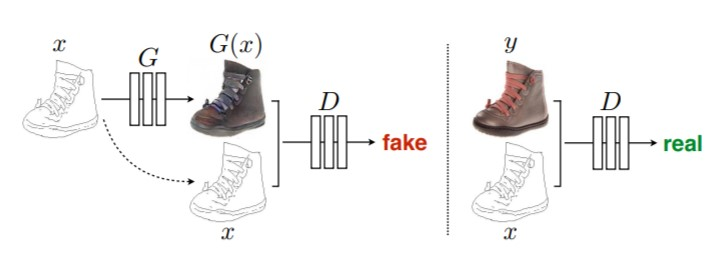
\includegraphics[width=0.5\linewidth]{fig/4.jpg}
    \caption{訓練Conditional GAN將鞋子的邊緣圖生成實際鞋子的圖像。(取自\cite{isola2017image})}
    \label{fig:4}
\end{figure}

\begin{figure}[htbp]
    \centering
    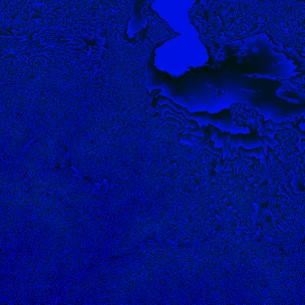
\includegraphics[width=0.5\linewidth]{fig/5.jpg}
    \caption{Encoder-decoder與U-Net結構比較 (取自\cite{isola2017image})}
    \label{fig:5}
\end{figure}



\subsubsection{VAE (Variational Autoencoder)}
Autoencoder模型為Encoder-decoder結構。運作時,輸入圖片x會被encoder編碼成latent code,再由decoder依照latent code的資訊嘗試還原出x。Latent code為整個模型結構的瓶頸,所以encoder的目標是把輸入x以最少資訊損失的方式壓縮成維數相對很小的latent code,以供decoder使用。也就是說,encoder做的是非線性降維,它會萃取輸入圖片的高階特徵。

而VAE(Variational Autoencoder)\cite{kingma2013auto}類似Autoencoder,但其中encoder的輸出為平均及標準差,這兩個參數代表著一個高斯(常態)分布,訓練時latent code會從該分布中隨機取出,傳給decoder。且latent code的先驗分布會被KL divergence限制在標準高斯分布內,這些限制使VAE能學到更有意義的latent space,也方便應用。

\begin{figure}[htbp]
    \centering
    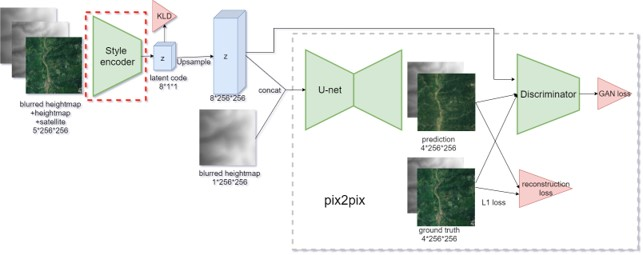
\includegraphics[width=0.45\linewidth]{fig/6.jpg}
    \caption{VAE的基本模型結構}
    \label{fig:6}
\end{figure}

生成擬真的人臉圖像即為VAE典型的應用,而VAE學習到的latent space中,各維度的意義可能是臉的方向、膚色、頭髮長度或眼睛大小。

我們的研究將以VAE與pix2pix結合,成為一種新的類神經網路架構,接著會利用這個類神經網路來訓練地形擬真模型和貼圖模型,最後會與基礎的pix2pix模型與物理侵蝕模型進行效果的比較。



\subsection{收集訓練模型所需之圖像資料}
本研究主要會收集五個地區的地形高度圖及空照圖。這個五個地區分別為橫斷山脈、喜馬拉雅山、祕魯安地斯山脈、阿根廷及加拿大的冰河地形。透過收集不同區域的地形,使VAE-pix2pix能學到不同地區的高度圖及空照圖的特徵。
\subsubsection{地形高度圖}
地形高度圖的資料來源為NASA的SRTM 1 Arc-Second資料集。此資料集將1經/緯度範圍的高度資料儲存為一張高度圖,每張高度圖的編號方式是按照其高度圖左下角的座標作為檔名,若此張高度圖的收集範圍為25°N, 98°E、25°N, 99°E、24°N, 99°E、24°N, 98°E四個座標點所圍成的範圍,則此張高度圖的檔名即為N24E98,我們在附錄中會使用這種方式來表示各地區的收集範圍。

因為SRTM資料集採用特殊的HGT格式,不能使用一般的圖像軟體讀取,也使得生成訓練資料集的工作變得麻煩,所以我們利用gmalthgtparser來將HGT格式轉為可以直接以圖像軟體讀取的PNG格式。gmalthgtparser為一個Python module,可以讀取HGT檔案中特定地點的高度值(單位為公尺),讀取到高度值後,我們利用式~\ref{eq:1}~將高度值轉為RGB值。

\begin{equation}
    (R, G, B)=\left(\left\lfloor\frac{\text {height}}{256^{2}}\right\rfloor,\left\lfloor\frac{\text {height } \% 256^{2}}{256^{1}}\right\rfloor,\left\lfloor\frac{\text {height } \% 256}{1}\right\rfloor\right)
    \label{eq:1}
\end{equation}

對高度值進行轉換後,我們即可以將一張HGT檔案的高度圖轉換為方便易用的PNG高度圖,轉換後的高度圖如圖~\ref{fig:7}~。

\begin{figure}[htbp]
    \centering
    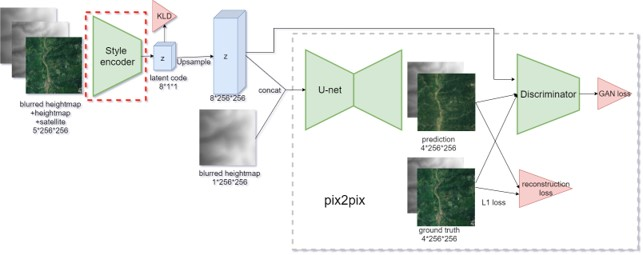
\includegraphics[width=0.45\linewidth]{fig/7.jpg}
    \caption{由hgt檔案轉換的PNG圖檔}
    \label{fig:7}
\end{figure}

\subsubsection{衛星空照圖}
本研究中,地形高度圖需要與衛星空照圖相互對應,所以使用MapTiler網站所提供的XYZ tiles map來收集衛星空照圖。XYZ tiles map是一種儲存地圖資料的方式,其方式為將大圖切割成許多張小圖,可以使地圖加載的速度變快,亦可節省網路資源。我們利用MapTiler所提供的衛星空照圖tiles map服務,收集橫斷山脈範圍內的多張衛星空照圖,再以EPSG:4326 (WGS 84)座標系統將各張小圖(tiles)組合成一張與地形高度圖互相對應的衛星空照圖。

因為衛星空照圖需與地形高度圖相互對應,所以空照圖的收集數量要與高度圖相同。表~\ref{tab:2}~為收集五個地區的高度圖及空照圖數量,具體的收集範圍列於附錄A:

\begin{table}[htbp]
    \centering
    \caption{五個地區的高度圖及空照圖收集總數 (單位:張)}
    \begin{tabularx}{\linewidth}{|Y|Y|Y|}
        \hline
        地區           & 高度圖數量 & 空照圖數量 \\ \hhline{|=|=|=|}
        橫斷山脈       & 16         & 16         \\ \hline
        喜馬拉雅山     & 10         & 10         \\ \hline
        祕魯安地斯山   & 15         & 15         \\ \hline
        阿根廷冰河地形 & 9          & 9          \\ \hline
        加拿大冰河地形 & 5          & 5          \\ \hline
    \end{tabularx}
    \label{tab:2}
\end{table}
\subsection{pix2pix模型的訓練方式}
pix2pix模型之訓練方式是輸入一對照片,其中一張照片為輸入,另一張照片則為目標輸出。pix2pix模型的目標即是將模型輸出盡可能接近目標輸出。在訓練過程中,我們將訓練圖像集分為三個部分,分別為train、val及test,\textbf{train是用於訓練模型,val則是在訓練過程中驗證模型的正確性,test則是在訓練完成後,用於測試模型}。
\subsection{生成訓練資料集}
我們將收集的高度圖和空照圖分為train、val及test三個區域(如圖~\ref{fig:8}~),並分別從這三個區域中切割出訓練資料集的圖像,這樣可以使三個部分的圖像不重複,以測試模型的精準度。

\begin{figure}[htbp]
    \centering
    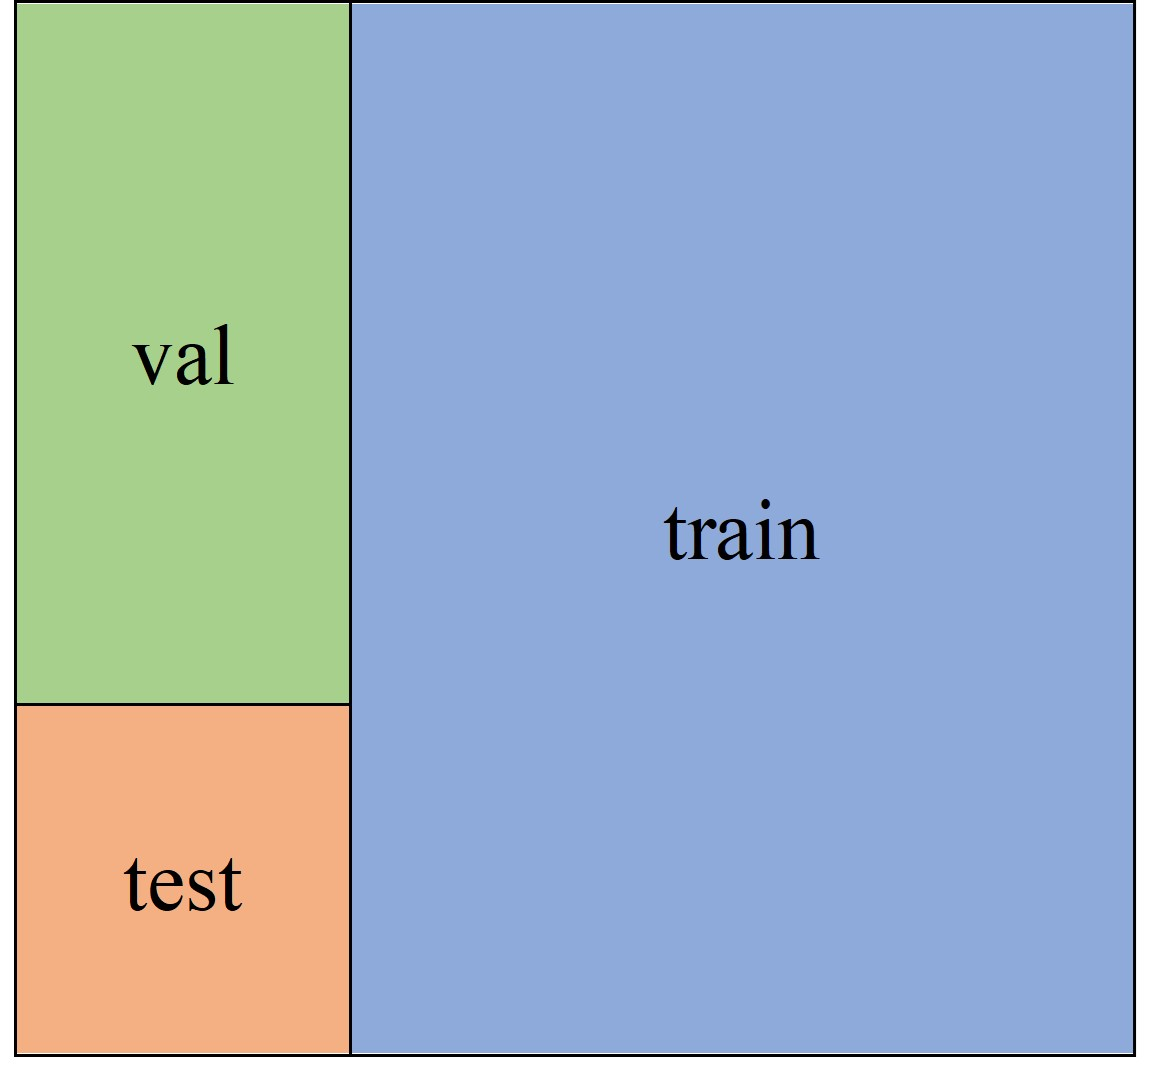
\includegraphics[width=0.3\linewidth]{fig/8.jpg}
    \caption{train、val、test在大圖的位置}
    \label{fig:8}
\end{figure}

\subsubsection{生成貼圖模型訓練資料集}
貼圖模型的目標是將輸入的空照圖生成相對應的高度圖,所以我們的訓練資料對即是空照圖及高度圖,其中空照圖為輸入(input),高度圖為目標輸出(ground truth)。

將圖片分割成上述的三個區域後,我們隨機在高度圖與空照圖上切割出多個$256 \times 256$大小的圖像,並將高度圖與空照圖拼接在一起,形成一個訓練資料對,如圖~\ref{fig:9}~。然後將五個地區的空照圖與高度圖一起放在同一個資料集,透過我們的模型訓練,學習到這五個地區的高度圖及空照圖中不同的特徵。

\begin{figure}[htbp]
    \centering
    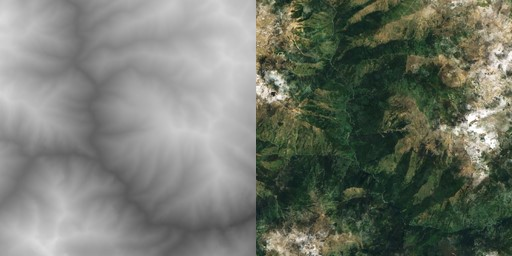
\includegraphics[width=0.5\linewidth]{fig/9.jpg}
    \caption{貼圖模型之訓練資料對}
    \label{fig:9}
\end{figure}

五個地區在train、val、test三個資料集中所佔的圖像數量皆相同,train為512張、val為128張、test為80張。所以整個資料集的train、val、test張數分別為2560張、640張、400張。

\subsubsection{生成地形擬真模型訓練資料集}

訓練的資料對共有兩張圖像,分別做為輸入及目標輸出。目標輸出圖片的生成方式是從先前蒐集的地形高度圖上隨機取$256 \times 256$大小的正方形。每次選取正方形的位置都是隨機的,以增進訓練資料的一般性。

至於輸入圖像,如果要用人工模仿每張目標輸出的方式畫出手繪圖,會花費很多時間。所以我們使用中值模糊的方式來快速生成輸入圖片。經過中值模糊處理後的圖片,在真實高度圖中的\textbf{大山脊上的小河谷}和\textbf{大河谷上的小凸起物}會被抹除,剩下的線條類似手繪圖的大致架構,符合模型輸入中山脈的大致架構這項條件。為了增進模型對於不同模糊程度的一般性,每張圖像的模糊程度是隨機的,也就是說中值模糊的kernel size是1\~ 29隨機的奇數。

最後,我們將中值模糊過的真實高度圖和原始的真實高度圖組成模糊-清晰資料對(如圖~\ref{fig:10}~),用來訓練地形擬真模型。訓練資料集的train、val、test圖像數量與貼圖模型的資料集相同,如表~\ref{tab:3}~。

\begin{figure}[htbp]
    \centering
    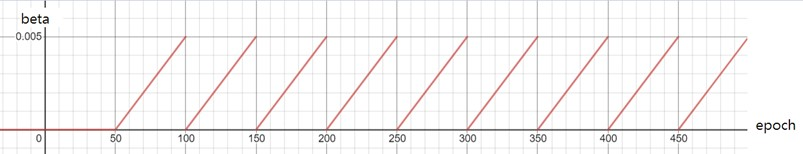
\includegraphics[width=0.5\linewidth]{fig/10.jpg}
    \caption{地形擬真模型之訓練資料對}
    \label{fig:10}
\end{figure}

\begin{table}[htbp]
    \centering
    \caption{貼圖模型與地形擬真模型的訓練資料的train、val、test圖像數量(單位:張)}
    \begin{tabularx}{\linewidth}{|Y|Y|Y|Y|Y|}
        \hline
        \textbf{模型的資料集} & \textbf{train}        & \textbf{val}         & \textbf{test}        & \textbf{總計}         \\ \hhline{|=|=|=|=|=|}
        貼圖模型              & \multirow{2}{*}{2560} & \multirow{2}{*}{640} & \multirow{2}{*}{400} & \multirow{2}{*}{3600} \\ \cline{1-1}
        地形擬真模型          &                       &                      &                      &                       \\ \hline
    \end{tabularx}
    \label{tab:3}
\end{table}

\subsection{本研究建構的模型結構 — VAE-pix2pix}
\label{subsec:5}
\subsubsection{貼圖模型}
本研究建構的模型為VAE及pix2pix的結合。pix2pix中的U-Net有強大的生成能力,負責依照高度圖生成空照圖。但是經過測試,我們發現如果只單獨提供高度圖給U-Net,它會無法反映出如雪線高度、山壁顏色等資訊。

為了解決這樣的問題,我們建構了VAE-pix2pix模型,在pix2pix的U-Net前增加了style encoder (為一個VAE),讓style encoder負責從目標空照圖提取出這些風格資訊,再由U-Net以正確的風格生成空照圖。從VAE的角度來看,此模型相當於利用U-Net作為Decoder,並在瓶頸處額外輸入高度圖作為空間資訊的VAE。\textbf{我們將建構的模型稱之為VAE-pix2pix模型}。

為了不限制能處理的圖片大小,本研究的style encoder不會像典型的VAE一樣產生向量作為latent code,而是會保留空間維度。

因為style encoder的輸入中含有目標空照圖(ground truth) 的資訊,所以作為瓶頸的latent code必須足夠窄,以防止U-Net輕易的將目標空照圖直接輸出。如果輸入圖的長寬為$256 \times 256$,則VAE會將latent code縮小到一個有16 channels,長寬為$4 \times 4$的tensor。貼圖模型的結構具體如圖~\ref{fig:11}~。

此外,模型中的style encoder中有使用Batch Normalization。本研究將batch size設為30,所以Batch Normalization不致於使style encoder輸出的latent code不穩定。

\begin{figure}[htbp]
    \centering
    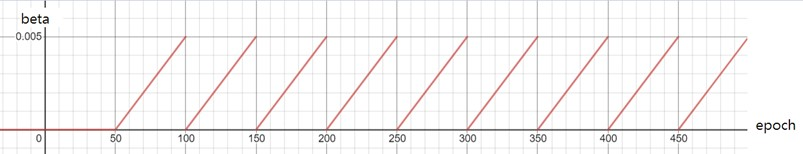
\includegraphics[width=\linewidth]{fig/11.jpg}
    \caption{貼圖模型的VAE-pix2pix模型結構}
    \label{fig:11}
\end{figure}

\subsubsection{地形擬真模型}
地形擬真模型結構和貼圖模型結構相同,差別只在地形擬真模型訓練時,是要以模糊高度圖做為輸入,藉以生成出較多細節的高度圖,而貼圖模型則是以清晰高度圖(ground truth)做為輸入。地形擬真模型的結構具體如圖~\ref{fig:12}~。

\begin{figure}[htbp]
    \centering
    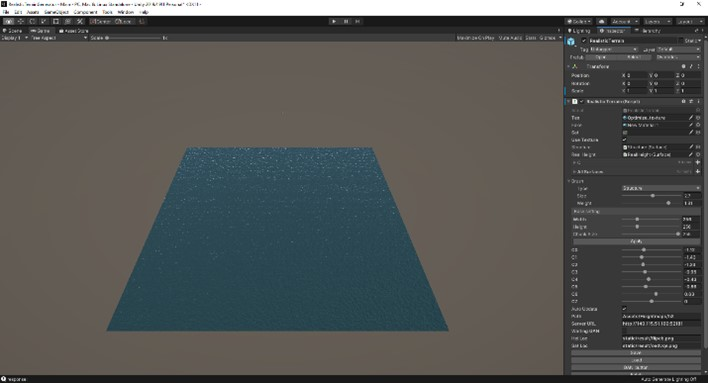
\includegraphics[width=\linewidth]{fig/12.jpg}
    \caption{貼圖模型的VAE-pix2pix模型結構}
    \label{fig:12}
\end{figure}

因本研究的模型結構是在pix2pix模型的基礎上額外加上VAE,所以pix2pix的部分仍然沿用論文作者的程式碼,進行訓練及測試時也是使用pix2pix原作者所提供的程式進行訓練及測試。
生成完貼圖模型的訓練資料集後,我們先訓練最基本的pix2pix模型。我們利用pix2pix模型所提供的train.py程式碼進行訓練,訓練指令如下:


\subsection{訓練貼圖模型}
生成完貼圖模型的訓練資料集後,我們先訓練最基本的pix2pix模型。我們利用pix2pix模型所提供的train.py程式碼進行訓練,訓練指令如下:

\begin{center}
    \texttt{\small python train.py --model pix2pix --name pix2pix\_sat\_all -–dataroot datasets/height29 \_10km\_pix2pix\_sat\_all --direction AtoB –-input\_nc 1 -–output\_nc 3}
\end{center}


\subsection{訓練VAE-pix2pix模型}
在~\textbf{\ref{subsec:5}\nameref{subsec:5}}~中提到我們是在pix2pix模型的架構下加入自行建構的VAE,故訓練指令與上述指令的差異只在model參數的不同,下述指令的vae\_pix2pix即為本研究的模型結構:

\begin{center}
    \texttt{\small python train.py --model vae\_pix2pix --name vae\_sat\_all -–dataroot datasets/height29 \_10km\_pix2pix\_sat\_all --direction AtoB –-input\_nc 1 -–output\_nc 3}
\end{center}

兩個貼圖模型的訓練結果會於\textbf{~\nameref{sec:res}~}中進行說明。

\subsection{訓練地形擬真模型}
在訓練原pix2pix模型與本研究建構的模型前,我們先對兩個模型內的pix2pix進行以下調整:
\subsubsection{對pix2pix模型進行調整}
pix2pix模型原本是針對「一般圖片的風格轉換」這項工作設計的,這裡指的是像素值有固定上下界且通常有RGB三數值的圖片。這和我們-「生成擬真山脈」性質上有些許不同,所以我們調整pix2pix模型使其符合需求(如圖~\ref{fig:13}~):
\begin{enumerate}
    \item 高度圖只有一個數值,所以設定模型的輸入(input\_nc)及輸出(output\_nc)維度皆為1。
    \item 高度圖的像素值沒有上下界的限制。為了讓輸出不因線性映射造成結果過大的失真,讓模型能均勻調整產生細節,我們把generator輸出層的激活函數(activation function) tanh去除。
    \item 將山脈加上細節和一般的風格轉換有很大的差別:前者的輸出會沿用輸入的像素「值」作為架構(不只沿用形狀架構),後者輸入和輸出的像素值則不必然有直接關係。所以我們在generator的最外層(也就是輸入和輸出層)加上額外的skip connection讓此層的輸出直接與模型輸入相加,成為最終的模型輸出(原本的generator第二層以下才有skip connection)。因此,模型只需要學習輸入和目標輸出的差,也就是哪裡要增高、哪裡要降低,而不用學習如何重建整個高度圖。
\end{enumerate}
\begin{figure}[htbp]
    \centering
    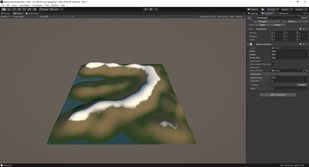
\includegraphics[width=0.6\linewidth]{fig/13.jpg}
    \caption{Generator(U-Net)的修改}
    \label{fig:13}
\end{figure}
\subsubsection{訓練pix2pix結構之地形擬真模型}
與貼圖模型相同,我們也利用pix2pix所提供的訓練程式碼來訓練模型,具體指令如下:
\begin{center}
    \texttt{\small python train.py --model pix2pix –-name pix2pix\_hei\_all\_med1-29 --dataroot datasets/height29\_10km\_pix2pix\_hei\_all\_med1-29 --direction AtoB –-input\_nc 1 -–output\_nc 1}
\end{center}
\subsubsection{訓練本研究模型結構之地形擬真模型}
而訓練本研究模型結構之地形擬真模型的具體指令如下:
\begin{center}
    \texttt{\small python train.py --model vae\_pix2pix -–name vae\_hei\_all --dataroot datasets/height29\_10km\_pix2pix\_sat\_all --direction AtoB –-input\_nc 1 -–output\_nc 3}
\end{center}

兩種地形擬真模型的訓練結果會於\textbf{~\nameref{sec:res}~}中進行探討。

\section{研究結果與討論}
\label{sec:res}
\subsection{評斷生成對抗網路模型的方法}
一般來說,很難找到一個好的方法來評斷生成對抗網路的表現,因為它不像一般的分類器能利用分類的精確度來評斷神經網路的優劣。

在本研究中,我們將會利用比較輸出與目標輸出的L1 Loss、L2 Loss、Perceptual Loss、FID、SSIM Index (structural similarity index)及生成每張圖像所需之平均時間來探討物理侵蝕模型、基礎的pix2pix模型與本研究模型的差異

\subsubsection{L1 Loss}
L1 Loss的計算方式是將兩張大小相同圖像所相對應的像素值相減後取絕對值,再相加在一起,最後取平均。具體公式如式~\ref{eq:2}~:
\begin{equation}
    \mathrm{L} 1 \operatorname{Loss}(X, Y)=\frac{1}{h \times w}\left(\sum_{i=1}^{h} \sum_{j=1}^{w}\left|X_{i, j}-Y_{i, j}\right|\right)
    \label{eq:2}
\end{equation}

其中,h, w分別為圖片的高度及寬度。可以發現L1 Loss的數值越小,代表兩張圖越相近。藉由L1 Loss我們可以看出兩張圖的相似程度。

\subsubsection{L2 Loss}
L2 Loss與L1 Loss的計算方式相似,只是將絕對值替換成平方,具體計算公式如式~\ref{eq:3}~:
\begin{equation}
    \mathrm{L} 2 \operatorname{Loss}(X, Y)=\frac{1}{h \times w}\left(\sum_{i=1}^{h} \sum_{j=1}^{w}\left(X_{i, j}-Y_{i, j}\right)^{2}\right)
    \label{eq:3}
\end{equation}

與L1 Loss相似,L2 Loss同樣是數值越小,代表兩張圖越相近,我們也可以透過L2 Loss來看出兩張圖的相似程度。但是L2 Loss對於偏離越多的值,會造成平方效果的改變。

\subsubsection{Perceptual Loss}

在計算Perceptual Loss\cite{zhang2018perceptual}時,會利用到一個已經訓練好(pre-trained)的VGG16模型。Perceptual Loss的計算方式是計算兩張圖像在VGG16各層activation的L1 Loss,最後再將各層計算出的L1 Loss相加。從Perceptual Loss可以看出兩張圖的風格是否相似,且Perceptual Loss同樣是數值越小,代表兩張圖越相近。

\subsubsection{FID (Fréchet Inception Distance)}
在計算FID (Fréchet Inception Distance)\cite{DOWSON1982450}時,會利用到一個已經訓練好 (pre-trained)的inception network v3神經網路來提取兩張圖片的特徵(feature)。圖片的特徵(為一個2048維的高階特徵)主要可以從inception network輸出層的前一層提取到。對於目標輸出,我們可以假設這個2048維向量是服從高斯分布。那由神經網路輸出的特徵應該也要服從高斯分布。所以我們知道生成對抗網路的目標是使這兩個分布的距離盡量接近。

而計算這兩個分布的距離等同於求目標輸出和輸出的2048維特徵的距離。數學上,如果想要計算兩個分布的距離,我們可以使用Fréchet distance來進行計算。

在計算上,我們會假設這兩個分布是服從高斯分布,且我們知道若一個隨機變數服從於高斯分布,則這個隨機變數可以使用高斯分布的標準差與平均表示,只要兩個分布的標準差和平均皆相同,則兩個分布相同。標準差和平均就是用來計算FID。但因為這裡我們要計算的是多維的向量,所以我們會使用平均和共變異數(covariance)矩陣來計算兩個分布的距離。而平均的維度是2048維,而共變異數矩陣就是一個2048 x 2048維的矩陣。有了以上的定義後,我們就可以使用式~\ref{eq:4}~來計算輸出與目標輸出的FID。


\begin{equation}
    \mathrm{FID}(X, Y)=\left\|\mu_{X}-\mu_{Y}\right\|_{2}^{2}+\operatorname{Tr}\left(\Sigma_{X}+\Sigma_{Y}-2\left(\Sigma_{X} \Sigma_{Y}\right)^{\frac{1}{2}}\right)
    \label{eq:4}
\end{equation}

\subsubsection{SSIM index (structural similarity index)}
SSIM指標\cite{wang2004image}是一種用來評斷兩張圖像相似程度的方法,相較於其他種方法SSIM指標能更好的符合人眼對圖像品質的判斷。
SSIM指標主要透過比較兩張圖片的亮度、對比度及結構(structure)來評斷兩張圖片的相似程度,具體計算方式如式~\ref{eq:5}~:
\begin{equation}
    \begin{array}{l}
        \operatorname{SSIM}(\mathbf{X}, \mathbf{Y})=[l(\mathbf{X}, \mathbf{Y})]^{\alpha}[c(\mathbf{X}, \mathbf{Y})]^{\beta}[s(\mathbf{X}, \mathbf{Y})]^{\gamma}, \\
        l(\mathbf{X}, \mathbf{Y})=\frac{2 \mu_{x} \mu_{y}+c_{1}}{\mu_{x}^{2}+\mu_{y}^{2}+c_{1}}, c(\mathbf{X}, \mathbf{Y})=\frac{2 \sigma_{x} \sigma_{y}+C_{2}}{\sigma_{x}^{2}+\sigma_{y}^{2}+C_{2}}, s(\mathbf{X}, \mathbf{Y})=\frac{\sigma_{x y}+C_{3}}{\sigma_{x} \sigma_{y}+c_{3}}
    \end{array}
    \label{eq:5}
\end{equation}
$l(X,Y)$是用來比較$X$, $Y$兩張圖的亮度,$c(X,Y)$則是用來比較對比度,而$s(X,Y)$用來比較兩張圖的結構。$\mu_x,\mu_y$代表兩張圖像素值的平均,$\sigma_x,\sigma_y$代表兩張圖像素值的標準差,$\sigma_{xy}$為兩張圖的共變異數(covariance),$C_1,C_2,C_3$是三個常數,以避免出現分母0的情況。另外,在本研究中,我們設定$\alpha=\beta=\gamma=1$。

根據以上的公式,我們可以發現SSIM index滿足對稱性($\operatorname{SSIM}(X,Y)=\operatorname{SSIM}(Y,X)$)、有界性($-1\leq \operatorname{SSIM}(X,Y)\leq 1$)及極限值唯一($\operatorname{SSIM}(X,Y)=1 \Longleftrightarrow X=Y$)

\subsubsection{生成每張圖像所需的平均時間}

我們利用PyTorch內建的\texttt{torch.cuda.Event()}來計算生成圖像所需的時間。計算完生成總時間後,就可以算出生成單張圖像所需的平均時間。在本研究中,我們是利用一張Nvidia GTX 1080 Ti 12 GB的顯示卡來進行圖像的生成。

\subsection{貼圖模型之訓練結果}

表~\ref{tab:4}~為原pix2pix結構與VAE-pix2pix結構的貼圖模型的測試結果,其圖像皆為來自test資料集之圖像,也就是說模型並沒有在訓練過程中“看過”這些圖像。藉由觀察這些圖像,我們可以更好的評斷模型的學習程度。表~\ref{tab:5}~則為兩個模型在test資料集的平均指標值。

\begin{table}[htbp]
    \centering
    \caption{原pix2pix結構及VAE-pix2pix結構的貼圖模型的測試結果}
    \label{tab:4}
    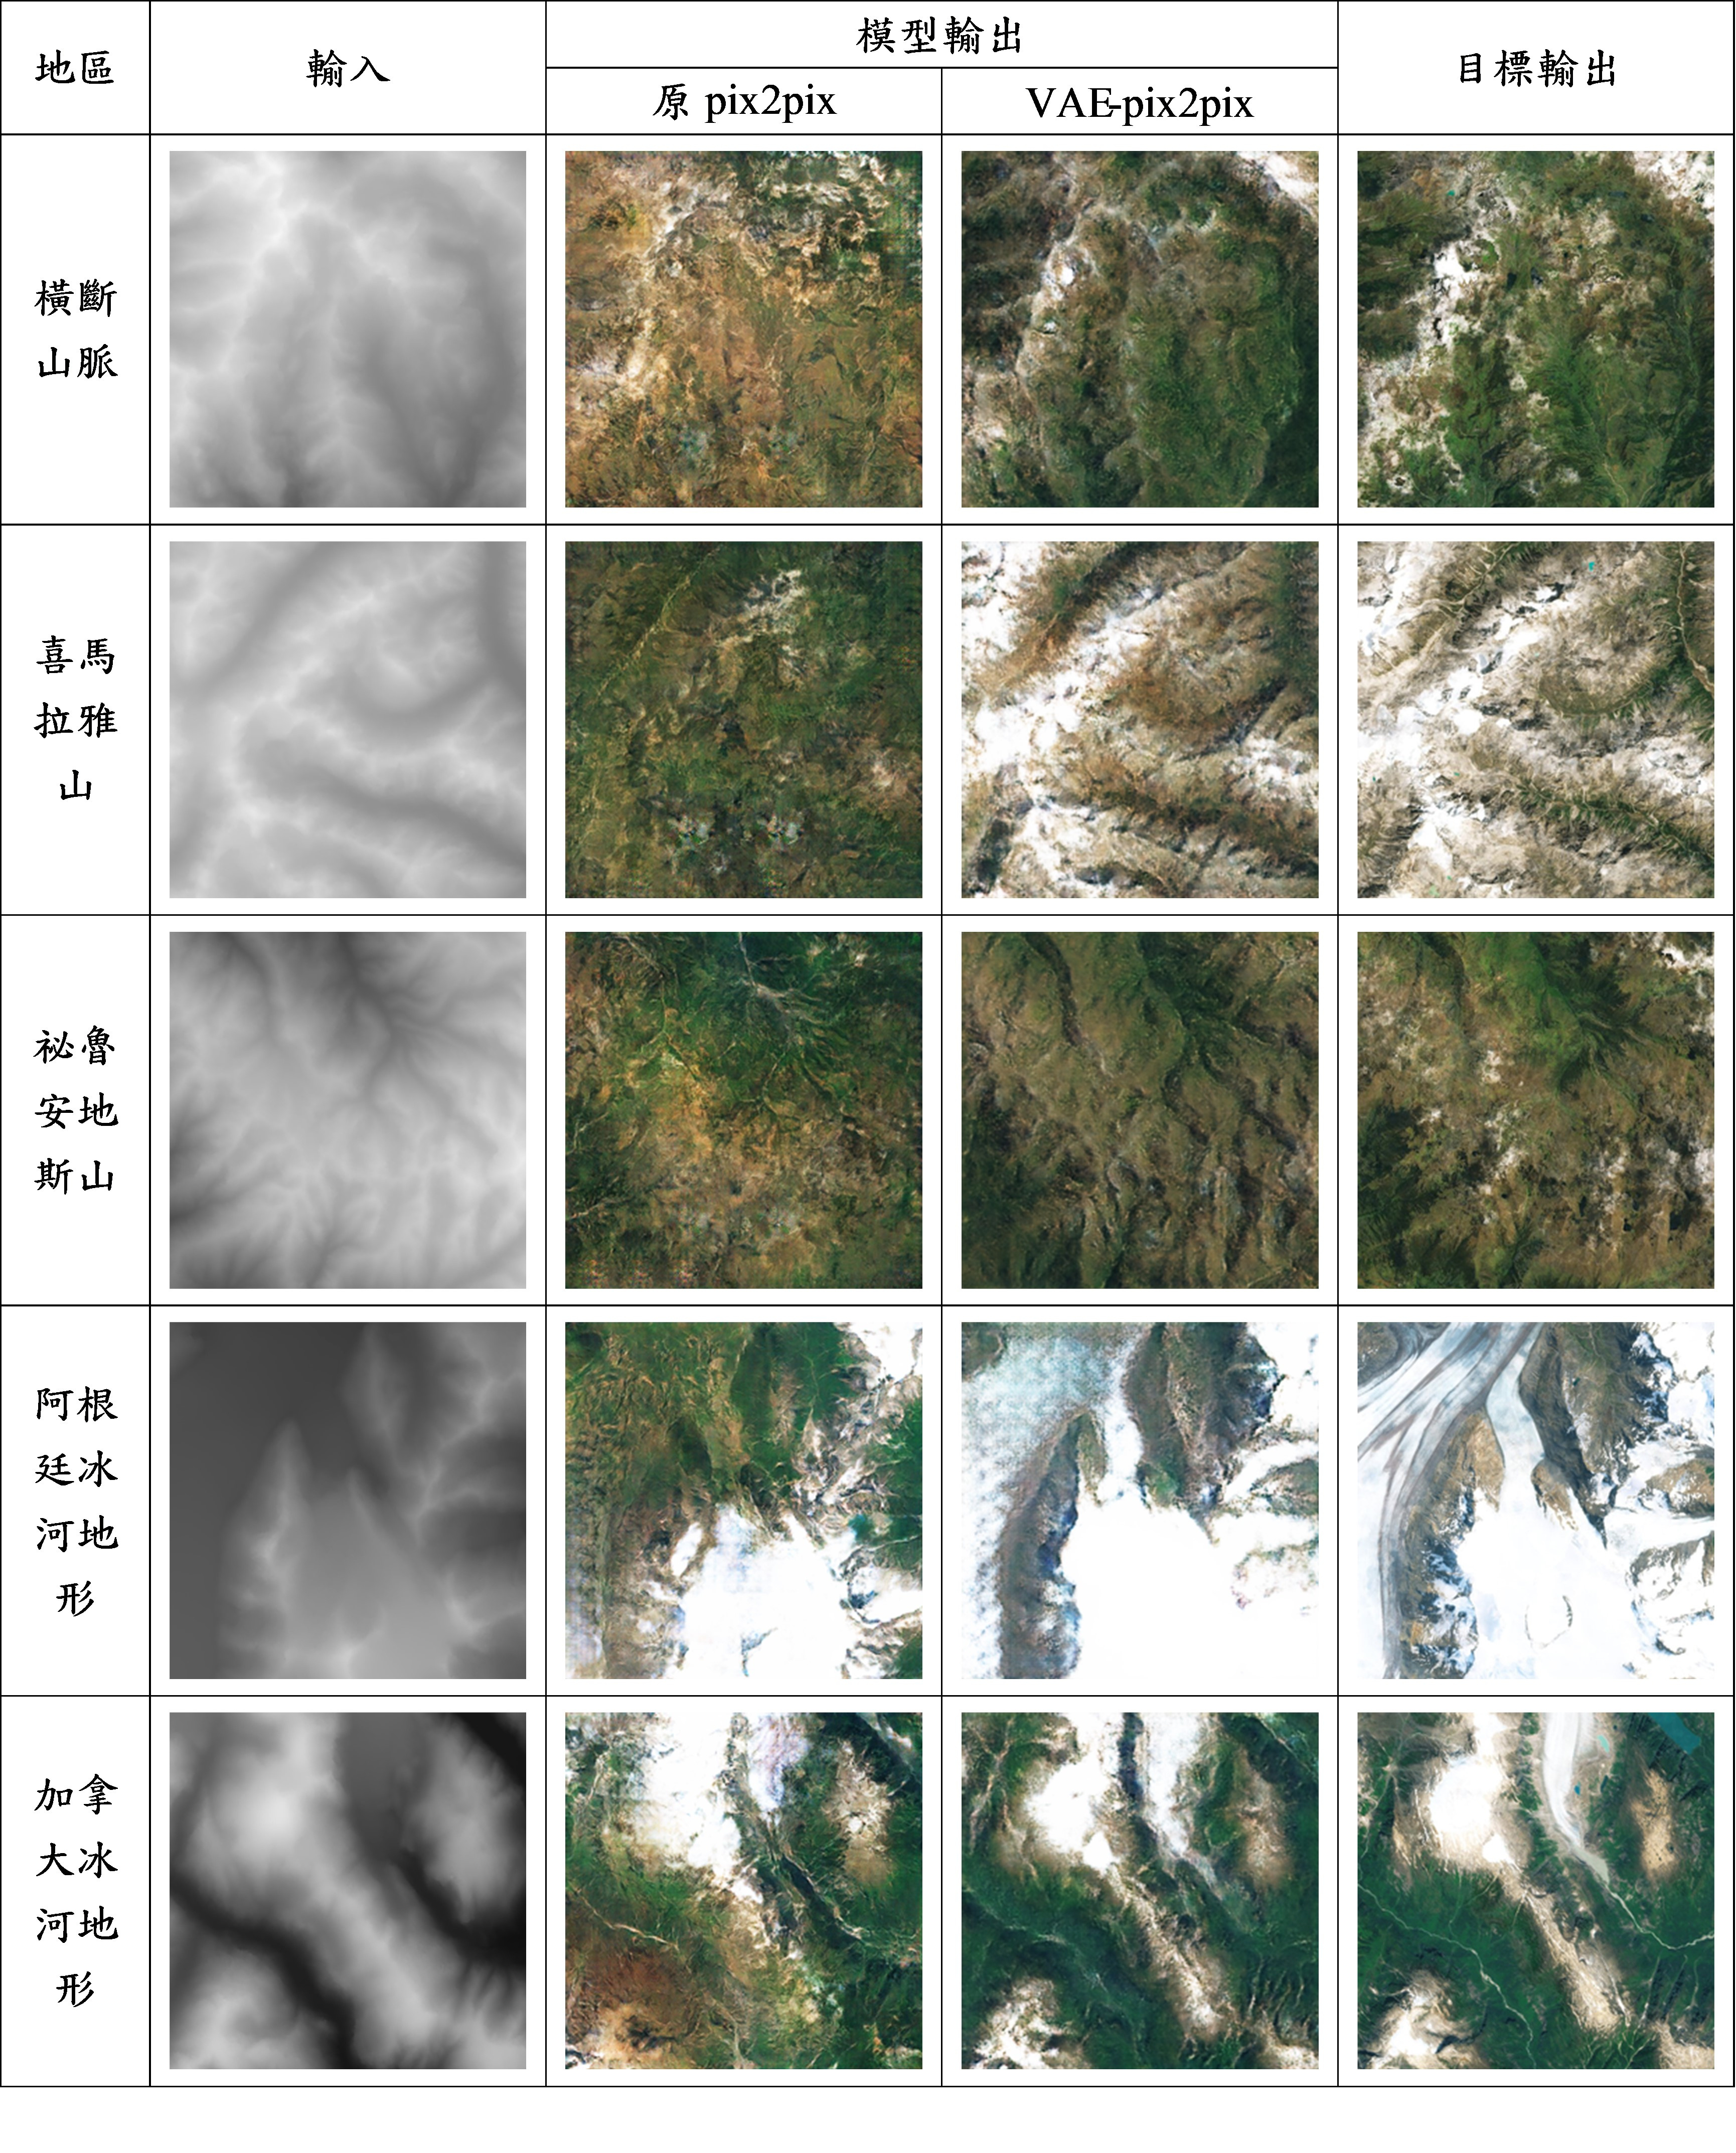
\includegraphics[width=0.8\linewidth]{fig/tab4.jpg}
\end{table}

\begin{table}[htbp]
    \caption{原pix2pix及VAE-pix2pix在test資料集的平均指標值}
    \label{tab:5}
    \begin{tabularx}{\linewidth}{|Y|Y|Y|Y|Y|Y|Y|}
        \hline
        \textbf{模型} & \textbf{L1 Loss} & \textbf{L2 Loss} & \textbf{Perceptual Loss} & \textbf{FID}    & \textbf{SSIM} & \textbf{平均生成時間(毫秒)} \\ \hhline{|=|=|=|=|=|=|=|}
        原pix2pix     & 44.17            & 3879.938         & 3.4326                   & \textbf{85.536} & 0.195         & \textbf{7.007}              \\ \hline
        VAE-pix2pix   & \textbf{18.466}  & \textbf{798.316} & \textbf{2.8969}          & 96.251          & \textbf{0.37} & 10.052                      \\ \hline
    \end{tabularx}
\end{table}


從表~\ref{tab:5}~可以發現我們建構的VAE-pix2pix架構相較於原pix2pix架構生成出的衛星空照圖較接近於目標輸出,不僅山脈的顏色更接近於目標輸出,且輸出的空照圖相當符合輸入高度圖的結構。這點也反映在各指標上,L1 Loss、L2 Loss、Perceptual Loss及SSIM都表現較好。
\subsection{地形擬真模型之訓練結果}
與貼圖模型相同,地形擬真模型的測試圖像都是來自test資料集。測試完成後,測試結果如表~\ref{tab:6}~,我們會將模型輸出與目標輸出計算出各指標,如表~\ref{tab:7}~,藉此來判斷每個模型的表現。
\begin{table}[htbp]
    \centering
    \caption{物理侵蝕模型、原pix2pix結構及VAE-pix2pix結構的地形擬真模型的測試結果}
    \label{tab:6}
    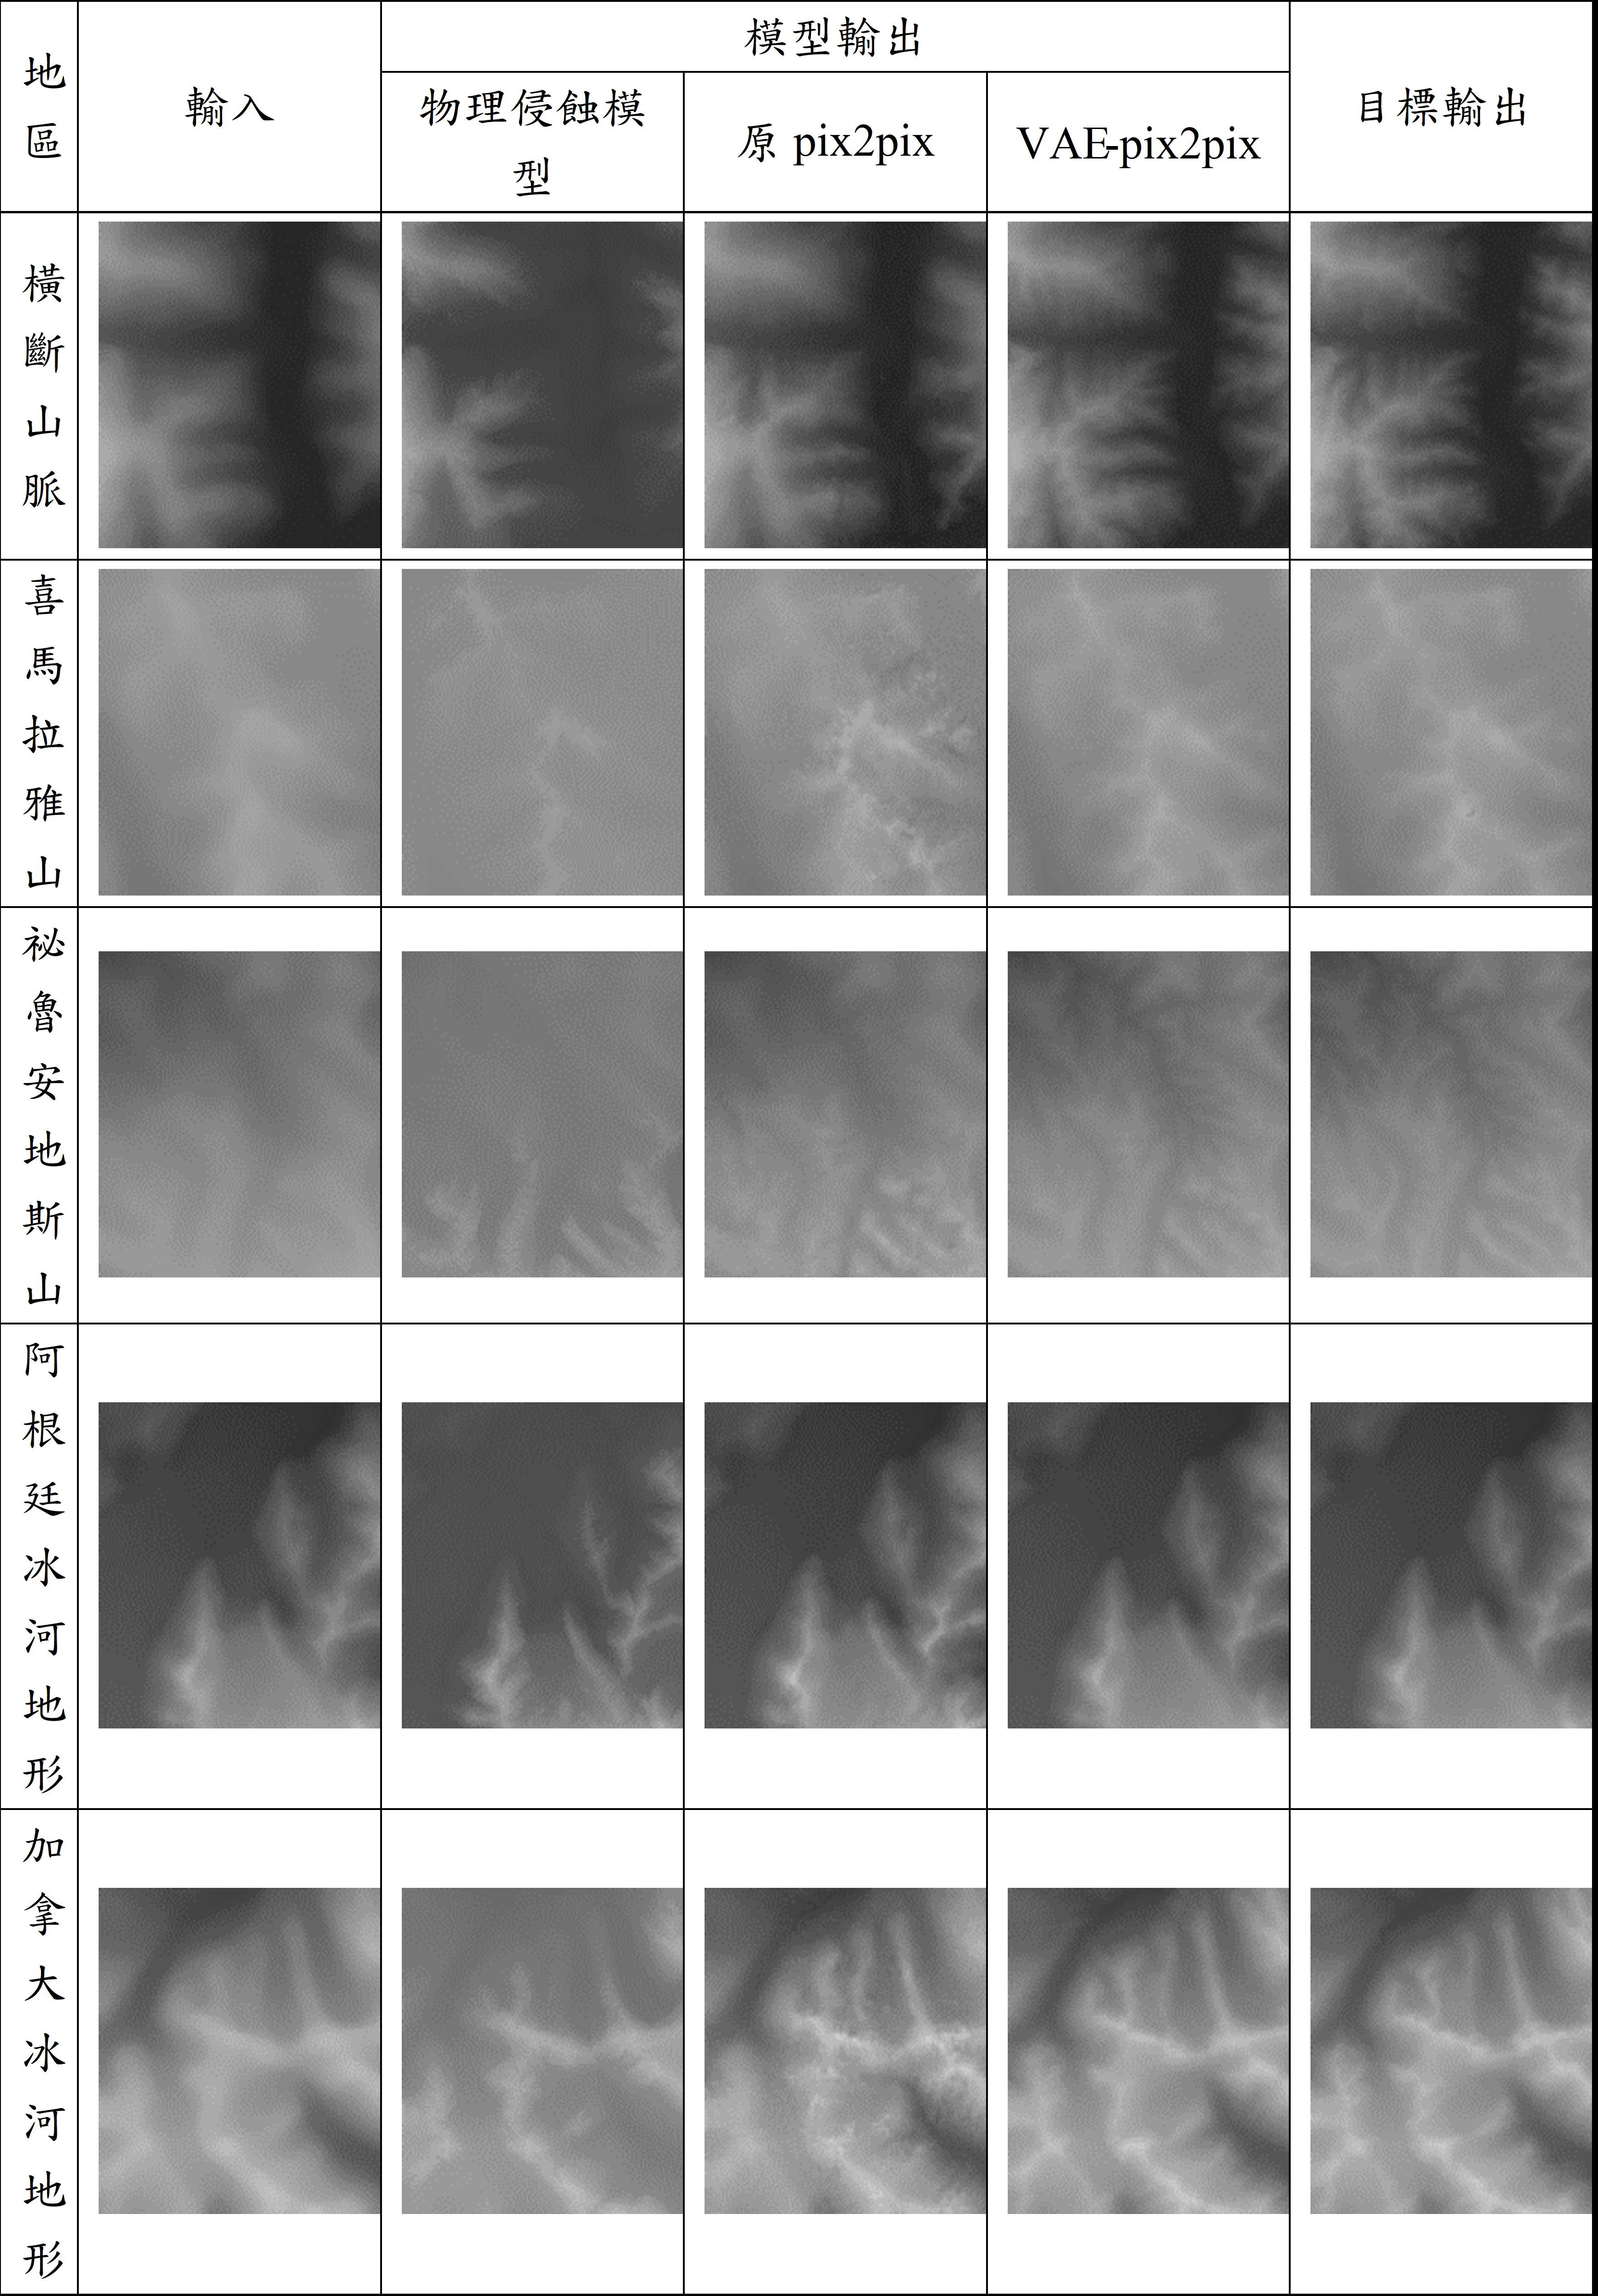
\includegraphics[width=0.9\linewidth]{fig/tab6.jpg}
\end{table}

\begin{table}[htbp]
    \caption{物理侵蝕模型、原pix2pix及VAE-pix2pix在test資料集的平均指標值}
    \label{tab:7}
    \begin{tabularx}{\linewidth}{|Y|Y|Y|Y|Y|Y|Y|}
        \hline
        \textbf{模型} & \textbf{L1 Loss} & \textbf{L2 Loss} & \textbf{Perceptual Loss} & \textbf{FID}    & \textbf{SSIM}  & \textbf{平均生成時間(毫秒)} \\ \hhline{|=|=|=|=|=|=|=|}
        物理侵蝕模型  & 9.735            & 157.747          & 0.7734                   & 144.036         & 0.897          & 1770                        \\ \hline
        原pix2pix     & 2.837            & 196.875          & 0.8327                   & 100.7692        & 0.931          & \textbf{7.863}              \\ \hline
        VAE-pix2pix   & \textbf{1.036}   & \textbf{9.413}   & \textbf{0.424}           & \textbf{33.742} & \textbf{0.982} & 10.247                      \\ \hline
    \end{tabularx}
\end{table}
從表~\ref{tab:7}~,我們可以發現VAE-pix2pix生成的高度圖較原pix2pix所生成的圖像來說更接近於目標輸出。由各指標也可以看到VAE-pix2pix要優於pix2pix。相較於物理侵蝕模型,我們的方法約比其生成的速度快20倍。
\subsection{將VAE-pix2pix的latent code進行PCA (主成分分析)}
在應用時,地形擬真模型和貼圖模型中的U-Net各需要輸入16維的latent code作為指定的生成風格。為了方便應用,我們將兩種模型在資料集中的所有圖片產生的latent code合併後進行PCA,這樣在使用時,使用者只需要輸入較少維的值(例如在Unity客戶端中為4維),再用PCA得到的轉換矩陣將它轉換到latent space,即可輸入U-Net。
\subsection{建構模型的API伺服器}
為了避免每次需要應用各模型處理高度圖時都要重新載入模型,我們利用Python的Flask套件建立了一個API伺服器,並將其建置於工作站上。用戶可以直接上傳高度圖,並在伺服器上用訓練好的各模型進行處理。這個API可以快速的在模型之間切換,且支援本研究中所有訓練的模型。
\subsection{Unity用戶端}
我們自行開發了一個Unity客戶端,使用戶可以在Unity Editor的編輯模式中直接對地形進行操作。使用者可以匯入一張高度圖或直接在地形上繪製3D的模型。每當畫完一筆畫後,Unity會直接對API伺服器送出請求,並在一秒內更新出擬真的山脈地形。也可以將貼圖模型所生成的擬真衛星空照圖貼在3D模型上,具體功能如圖~\ref{fig:14}~、圖~\ref{fig:15}~、圖~\ref{fig:16}~、圖~\ref{fig:17}~。



\begin{figure*}
    \centering
    \begin{subfigure}[b]{0.475\textwidth}
        \centering
        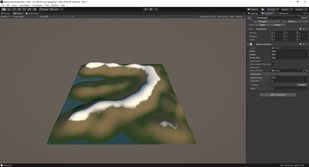
\includegraphics[width=\textwidth]{fig/14.jpg}
        \caption[]%
        {{\small Unity客戶端的初始畫面}}
        \label{fig:14}
    \end{subfigure}
    \hfill
    \begin{subfigure}[b]{0.475\textwidth}
        \centering
        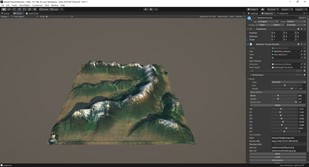
\includegraphics[width=\textwidth]{fig/15.jpg}
        \caption[]%
        {{\small 用戶手繪之大致地形}}
        \label{fig:15}
    \end{subfigure}
    \vskip\baselineskip
    \begin{subfigure}[b]{0.475\textwidth}
        \centering
        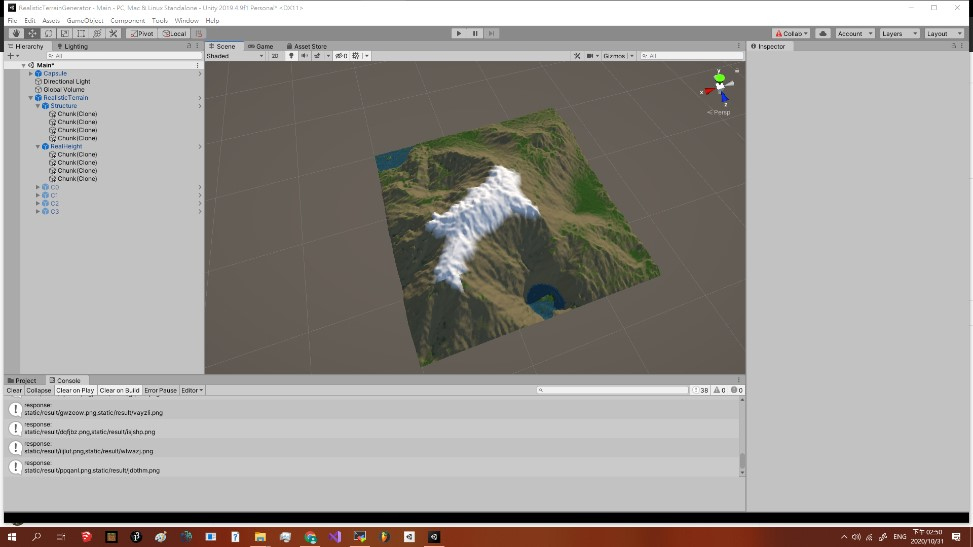
\includegraphics[width=\textwidth]{fig/16.jpg}
        \caption[]%
        {{\small 經過地形擬真模型處理後的擬真地形}}
        \label{fig:16}
    \end{subfigure}
    \hfill
    \begin{subfigure}[b]{0.475\textwidth}
        \centering
        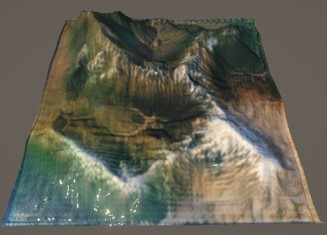
\includegraphics[width=\textwidth]{fig/17.jpg}
        \caption[]%
        {{\small 將貼圖模型的輸出貼在擬真地形上的效果}}
        \label{fig:17}
    \end{subfigure}
    \caption[ The average and standard deviation of critical parameters ]
    {\small Unity客戶端功能}
    \label{fig:unity}
\end{figure*}

\subsection{由用戶端調整latent code對於輸出風格的效果}
圖~\ref{fig:18}~展示了以$512 \times 512$的橫斷山脈模糊高度圖為輸入高度圖,並在空間上使用不同的latent code,造成模型輸出在空間上的風格差異。整張圖latent code的設置為:第一主成分由左邊界的-0.6線性增加至右邊界的0.6,第二主成分由下邊界的-0.6線性增加至上邊界的0.6,更後面的主成分皆設為0。

\begin{figure}[htbp]
    \centering
    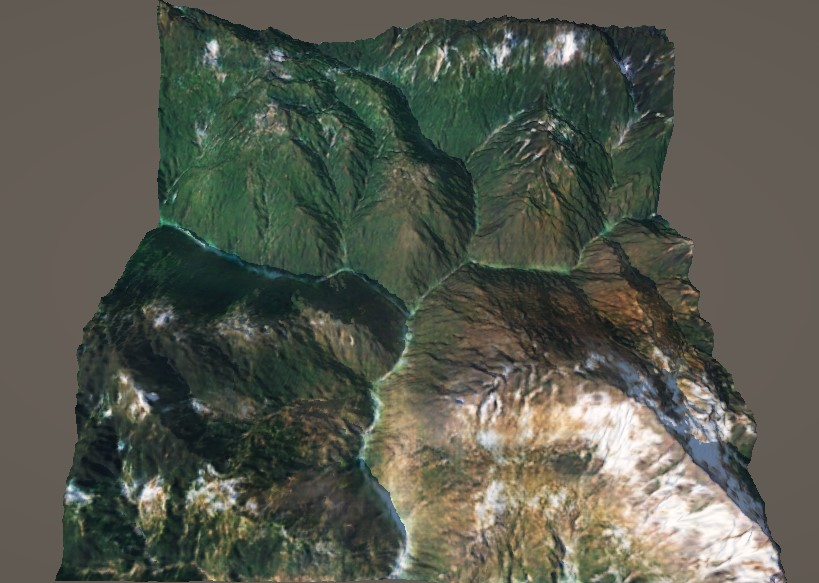
\includegraphics[width=0.7\linewidth]{fig/18.jpg}
    \caption{在空間上展示不同風格的輸出}
    \label{fig:18}
\end{figure}

\subsection{透過改變style encoder的輸入改變輸出圖像的風格}
為了測試以上的討論,我們將一張高度圖及多張與此張高度圖不互相對應的空照圖一起輸入到VAE-pix2pix的style encoder中,驗證能改變輸出圖像的風格。表~\ref{tab:8}~為測試的結果。
\begin{table}[htbp]
    \centering
    \caption{將同一張高度圖與不同的空照圖作為style encoder的輸入,並比較其輸出}
    \label{tab:8}
    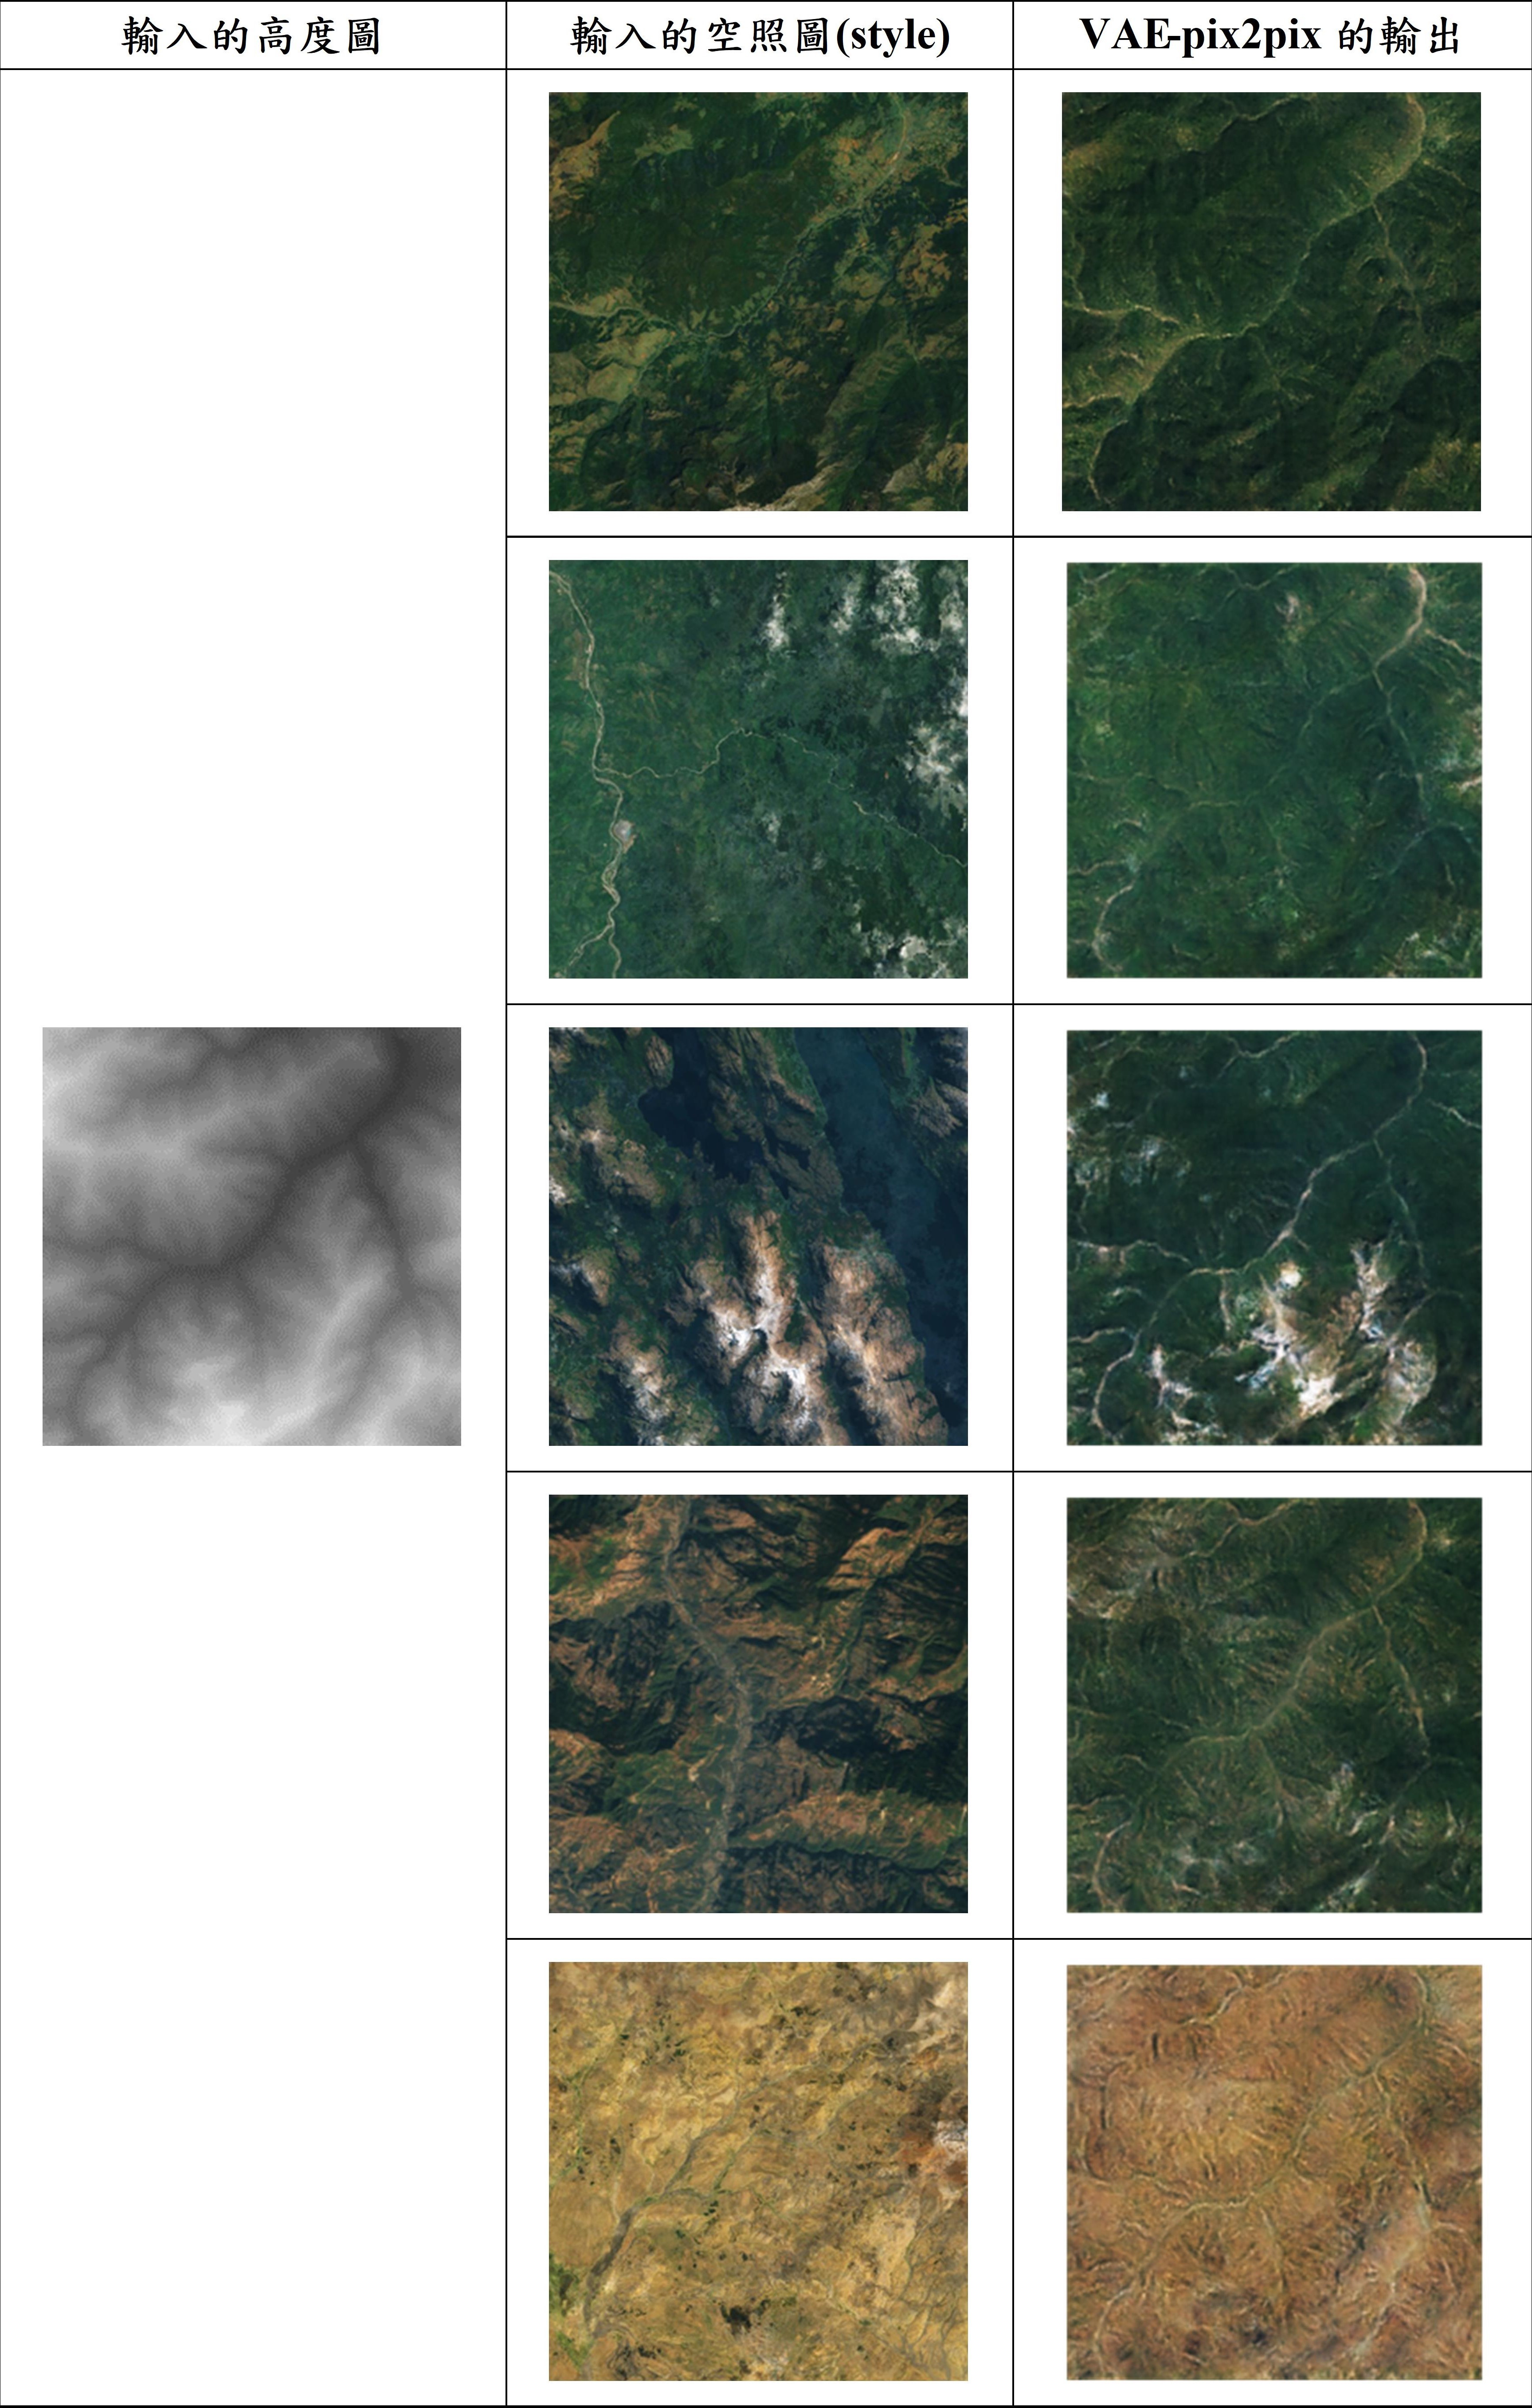
\includegraphics[width=0.8\linewidth]{fig/tab8.jpg}
\end{table}
可以發現VAE-pix2pix模型可以很好的將輸入空照圖的特徵提取出來,且也可以保留高度圖上河流及山脊等特徵。
\subsection{討論物理侵蝕模型、pix2pix模型及VAE-pix2pix之間的差異}
表~\ref{tab:9}~比較了物理侵蝕模型、原pix2pix模型及本研究建構的VAE-pix2pix模型之間的差異。

雖然VAE-pix2pix模型的生成速度慢於原pix2pix模型,但其所生成圖像的品質為三者最優,還可以透過改變latent code的數值,改變生成山脈地形的風格。
\begin{table}[htbp]
    \caption{物理侵蝕模型、原pix2pix模型及VAE-pix2pix的比較}
    \label{tab:9}
    \begin{tabularx}{\linewidth}{|Y|Y|Y|Y|Y|}
        \hline
        \textbf{模型}   & \textbf{功能}                                              & \textbf{生成速度} & \textbf{生成品質} & \textbf{是否可以改變生成圖像的風格} \\ \hhline{|=|=|=|=|=|}
        物理侵蝕模型    & 將大致高度圖經過侵蝕後變得較為擬真                         & 慢(約1.7秒)       & 最差              & 否                                  \\ \hline
        原pix2pix模型   & 將大致高度圖變得更為擬真、根據高度圖生成相對應的衛星空照圖 & 最快(約7毫秒)     & 其次              & 否                                  \\ \hline
        VAE-pix2pix模型 & 將大致高度圖變得更為擬真、根據高度圖生成相對應的衛星空照圖 & 快 (約10毫秒)     & 最好              & 是                                  \\ \hline
    \end{tabularx}
\end{table}
\section{結論與應用}

在本研究,我們利用NASA的SRTM 1 Arc-Second及MapTiler網站收集了全球五個地區的高度圖及相對應的空照圖。利用這些收集的圖像,訓練了自行建構的VAE-pix2pix模型。VAE-pix2pix為Variational Autoencoder (VAE)及pix2pix結合的模型,可以將人工繪製的高度圖自動加上真實山脈應有的細節(包含尖銳的山脊、山壁上的紋路、連續的河流網路等……),也能生成相對應的擬真衛星空照圖。

經過實測,相較於原pix2pix模型,VAE-pix2pix所生成的高度圖及空照圖會更接近於真實世界的山脈高度圖,且VAE-pix2pix模型也可以透過改變其latent code的數值來生成出不同風格的高度圖及衛星空照圖,如地貌的顏色或雪線的高度等,這些都能增加模型生成圖像的多樣性,讓應用更為廣泛。與物理侵蝕模型進行比較,不僅生成速度遠快於物理侵蝕模型,生成品質也更為擬真,這些優於傳統模型的地方。

為了使模型的使用更加簡單,不用在終端機上打入許多複雜的指令,我們將模型的使用包裝成Unity客戶端,Unity客戶端可以在圖形使用者介面完成在模糊高度圖加上山脈細節的工作,並能直接在畫面上顯示3D模型,也可以將生成出的衛星空照圖貼在擬真地形的3D模型中,使空照圖及高度圖能更好的呈現。

綜合以上,本研究的VAE-pix2pix模型可以生成出更為擬真的高度圖及空照圖。而我們開發的Unity客戶端,可以使我們的模型直接應用於遊戲的開發中,也使得原先需要分成兩個步驟的生成擬真的山脈地形與生成相對應的空照圖整合為一個步驟。這些都會讓遊戲開發生成擬真山脈模型的任務變得十分容易。

\nocite{*}
\printbibliography[title={參考文獻}]

\addcontentsline{toc}{section}{參考文獻}


\newpage
\begin{appendices}
    \setcounter{page}{1}
    \textbf{\LARGE 附錄}

    \section{VAE-pix2pix的模型結構}
    \begin{center}
        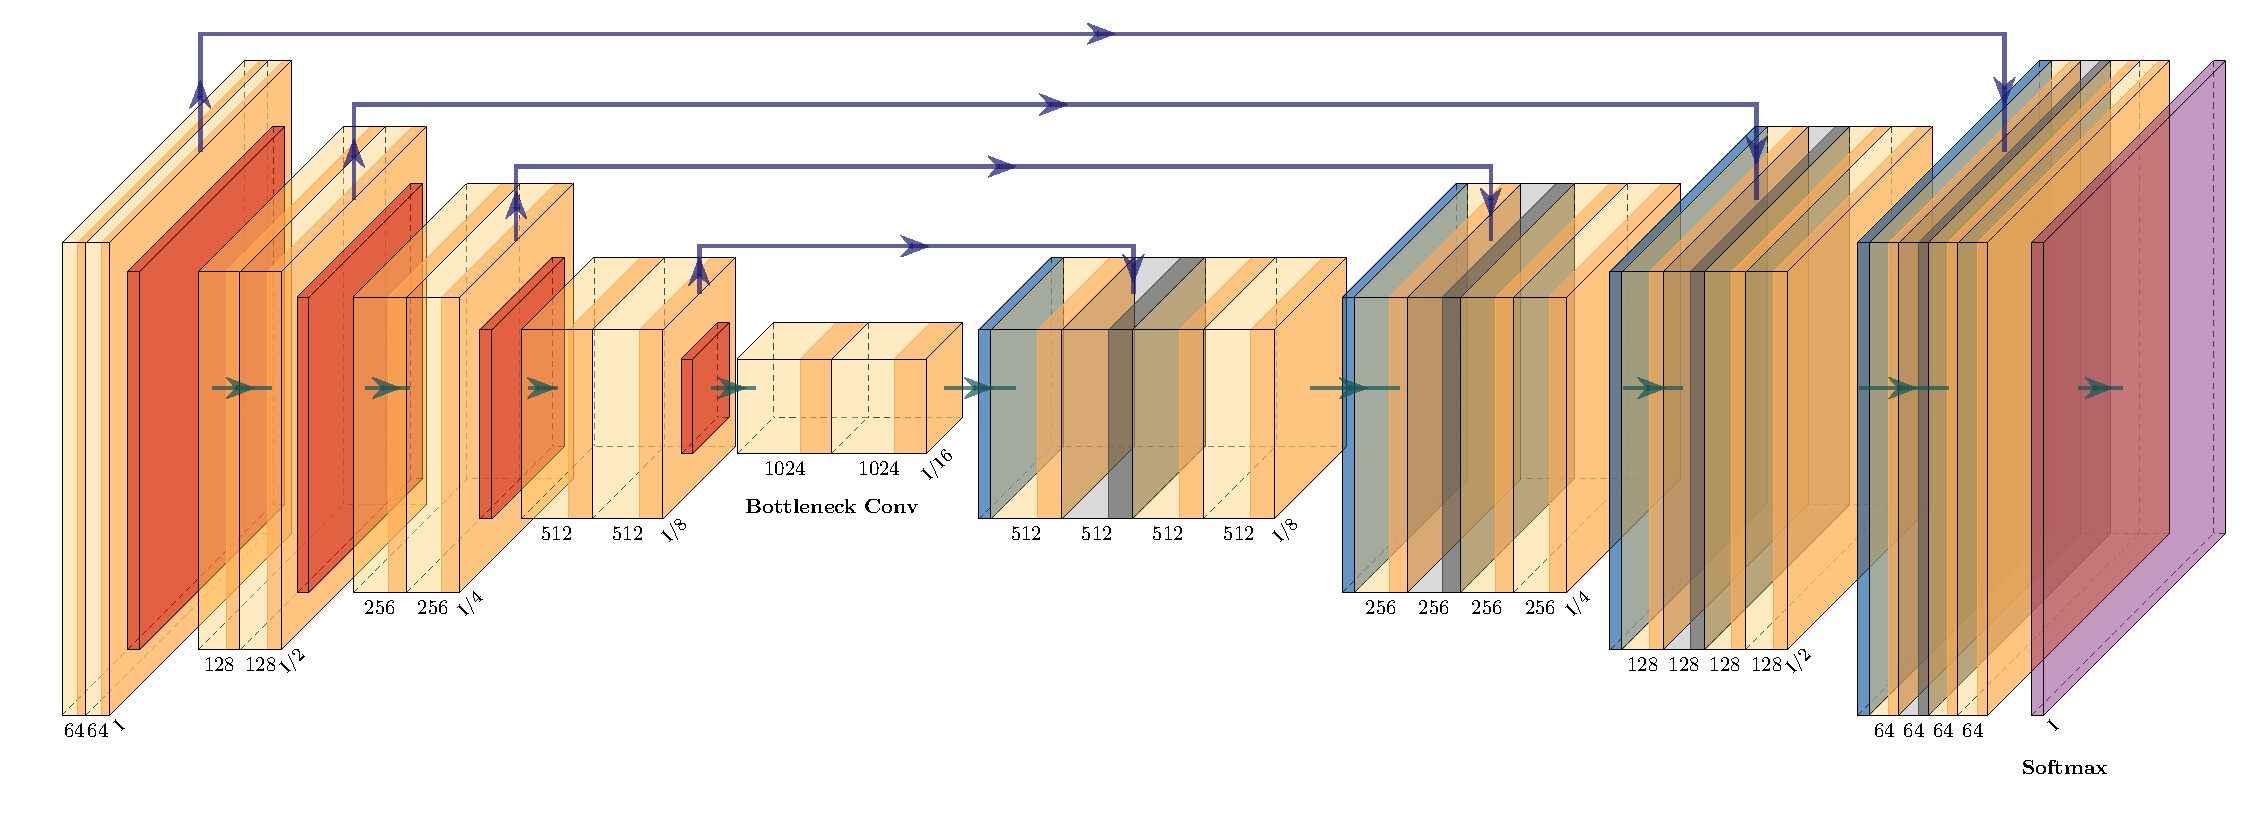
\includegraphics[width=\textwidth]{fig/Unet.pdf}
    \end{center}

    \section{高度圖及空照圖的具體收集範圍}
    如內文所提,我們會利用高度圖左下角的經緯度座標表示一張高度/空照圖,如一張高度圖是由25°N, 98°E、25°N, 99°E、24°N, 99°E、24°N, 98°E四個座標點所圍成的範圍,則此張高度圖的檔名即為N24E98。除了會在下面列出各個座標點,我們也有將具體的收集範圍在地圖上框出。

    \subsection{中國橫斷山脈}
    \begin{multicols}{4}
        \begin{enumerate}
            \item N27E099
            \item N27E098
            \item N26E101
            \item N26E100
            \item N26E099
            \item N26E098
            \item N29E101
            \item N29E100
            \item N29E099
            \item N29E098
            \item N28E101
            \item N28E100
            \item N28E099
            \item N28E098
            \item N27E101
            \item N27E100
        \end{enumerate}
    \end{multicols}
    \begin{figure}[H]
        \centering
        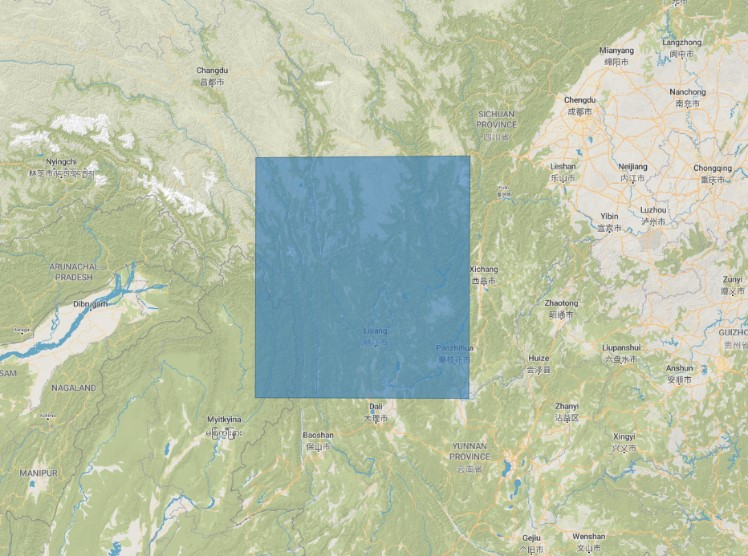
\includegraphics[width=0.8\linewidth]{fig/a1.jpg}
    \end{figure}
    \subsection{喜馬拉雅山脈}
    \begin{multicols}{4}
        \begin{enumerate}
            \item N29E081
            \item N29E082
            \item N29E083
            \item N28E083
            \item N28E084
            \item N28E085
            \item N27E085
            \item N27E086
            \item N28E086
            \item N27E087
        \end{enumerate}
    \end{multicols}
    \begin{figure}[H]
        \centering
        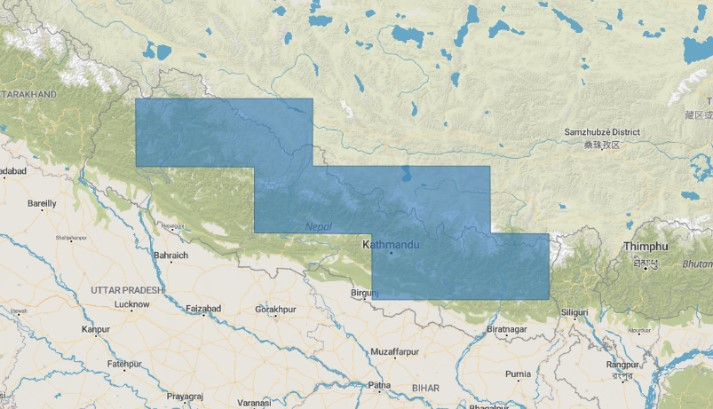
\includegraphics[width=0.8\linewidth]{fig/a2.jpg}
    \end{figure}
    \subsection{祕魯安地斯山脈}
    \begin{multicols}{4}
        \begin{enumerate}
            \item S07W079
            \item S08W079
            \item S08W078
            \item S09W078
            \item S10W078
            \item S10W077
            \item S11W077
            \item S12W077
            \item S12W076
            \item S13W076
            \item S14W076
            \item S14W075
            \item S15W075
            \item S15W074
            \item S16W073
        \end{enumerate}
    \end{multicols}
    \begin{figure}[H]
        \centering
        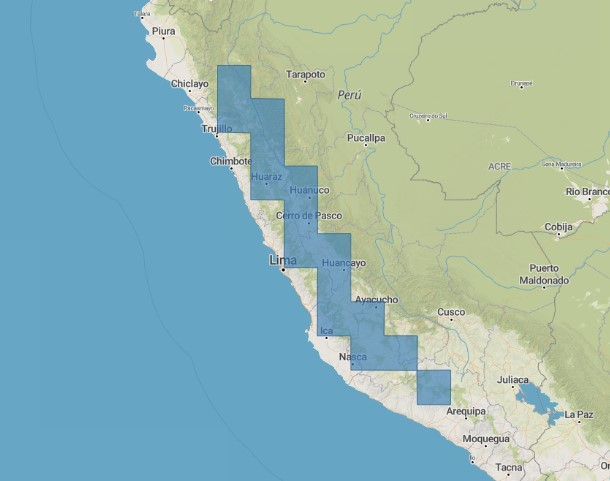
\includegraphics[width=0.8\linewidth]{fig/a3.jpg}
    \end{figure}
    \subsection{阿根廷冰河}
    \begin{multicols}{3}
        \begin{enumerate}
            \item S48W074
            \item S49W074
            \item S49W075
            \item S50W074
            \item S50W075
            \item S51W073
            \item S51W074
            \item S51W075
            \item S52W074
        \end{enumerate}
    \end{multicols}
    \begin{figure}[H]
        \centering
        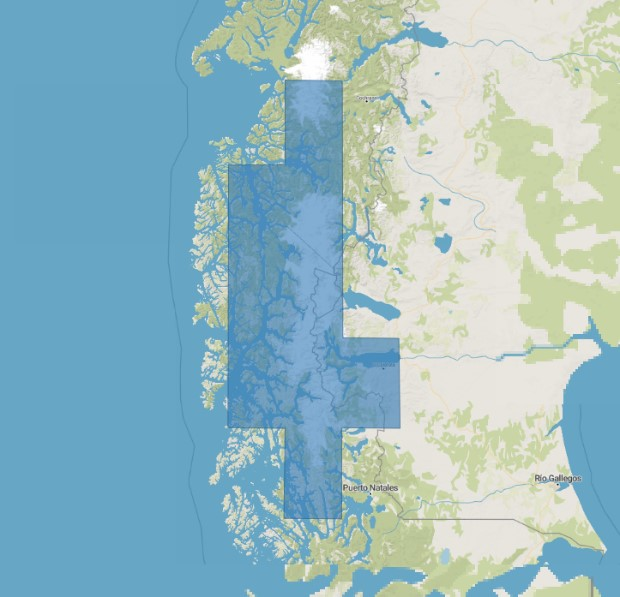
\includegraphics[width=0.8\linewidth]{fig/a4.jpg}
    \end{figure}
    \subsection{加拿大冰河}
    \begin{multicols}{3}
        \begin{enumerate}
            \item N58W134
            \item N57W133
            \item N56W132
            \item N56W131
            \item N55W131
        \end{enumerate}
    \end{multicols}
    \begin{figure}[H]
        \centering
        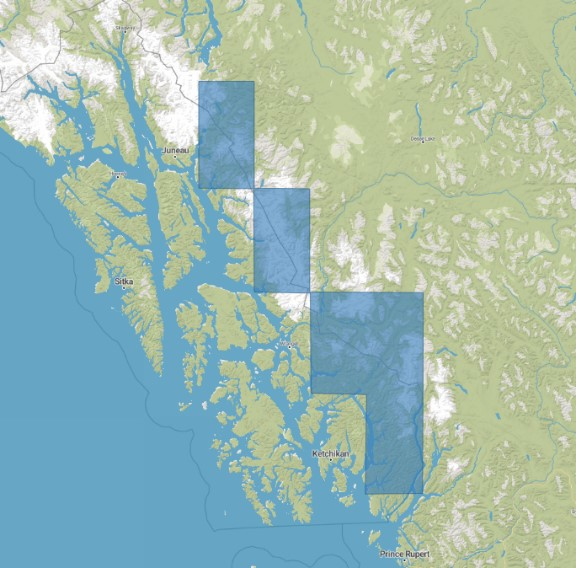
\includegraphics[width=0.8\linewidth]{fig/a5.jpg}
    \end{figure}
\end{appendices}

\end{document}